\documentclass[12pt,dvipdfmx]{beamer}
\usepackage{graphicx}
\DeclareGraphicsExtensions{.pdf}
\DeclareGraphicsExtensions{.eps}
\graphicspath{{out/tex/lsvg/}{out/tex/svg/}{out/pdf/svg/}}

\usepackage{listings}
\usepackage{fancybox}
\usepackage{hyperref}
\usepackage{color}

\newcommand{\plusequal}{\mbox{\tt\ += }}
\newcommand{\minusequal}{\mbox{\tt\ -= }}
\newcommand{\divequal}{\mbox{\tt\ /= }}
\newcommand{\plusplus}{\mbox{\tt\ ++ }}



%% OpenMP section numbers
\newcommand{\sectionompparallel}{2.5}
\newcommand{\sectionompdeterminenumthreads}{2.5.1}
\newcommand{\sectionompfor}{2.7.1}
\newcommand{\sectionompdataenv}{2.14}
\newcommand{\sectionompgetnumthreads}{3.2.2}
\newcommand{\sectionompgetmaxthreads}{3.2.3}
\newcommand{\sectionompgetthreadnum}{3.2.4}


%%%%%%%%%%%%%%%%%%%%%%%%%%%
%%% themes
%%%%%%%%%%%%%%%%%%%%%%%%%%%
%\usetheme{Szeged} 
\usetheme{Madrid}

%% no navigation bar
% default boxes Bergen Boadilla Madrid Pittsburgh Rochester
%% tree-like navigation bar
% Antibes JuanLesPins Montpellier
%% toc sidebar
% Berkeley PaloAlto Goettingen Marburg Hannover Berlin Ilmenau Dresden Darmstadt Frankfurt Singapore Szeged
%% Section and Subsection Tables
% Copenhagen Luebeck Malmoe Warsaw

%%%%%%%%%%%%%%%%%%%%%%%%%%%
%%% innerthemes
%%%%%%%%%%%%%%%%%%%%%%%%%%%
% \useinnertheme{circles}	% default circles rectangles rounded inmargin

%%%%%%%%%%%%%%%%%%%%%%%%%%%
%%% outerthemes
%%%%%%%%%%%%%%%%%%%%%%%%%%%
% outertheme
% \useoutertheme{default}	% default infolines miniframes smoothbars sidebar sprit shadow tree smoothtree


%%%%%%%%%%%%%%%%%%%%%%%%%%%
%%% colorthemes
%%%%%%%%%%%%%%%%%%%%%%%%%%%
\usecolortheme{seahorse}
%% special purpose
% default structure sidebartab 
%% complete 
% albatross beetle crane dove fly seagull 
%% inner
% lily orchid rose
%% outer
% whale seahorse dolphin

%%%%%%%%%%%%%%%%%%%%%%%%%%%
%%% fontthemes
%%%%%%%%%%%%%%%%%%%%%%%%%%%
\usefonttheme{serif}  
% default professionalfonts serif structurebold structureitalicserif structuresmallcapsserif

%%%%%%%%%%%%%%%%%%%%%%%%%%%
%%% generally useful beamer settings
%%%%%%%%%%%%%%%%%%%%%%%%%%%
% 
\AtBeginDvi{\special{pdf:tounicode EUC-UCS2}}
% do not show navigation
\setbeamertemplate{navigation symbols}{}
% show page numbers
\setbeamertemplate{footline}[frame number]


%%%%%%%%%%%%%%%%%%%%%%%%%%%
%%% define some colors for convenience
%%%%%%%%%%%%%%%%%%%%%%%%%%%

%\newcommand{\mido}[1]{{\color{green}#1}}
\newcommand{\mido}[1]{{\color{green}#1}}
\newcommand{\mura}[1]{{\color{purple}#1}}
\newcommand{\ore}[1]{{\color{orange}#1}}
\newcommand{\ao}[1]{{\color{blue}#1}}
\newcommand{\aka}[1]{{\color{red}#1}}

\setbeamercolor{ex}{bg=cyan!20!white}

%%%%%%%%%%%%%%%%%%%%%%%%%%%
%%% how to typset code
%%%%%%%%%%%%%%%%%%%%%%%%%%%

\lstset{language = C,
numbers = left,
numberstyle = {\tiny \emph},
numbersep = 10pt,
breaklines = true,
breakindent = 40pt,
frame = tlRB,
frameround = ffft,
framesep = 3pt,
rulesep = 1pt,
rulecolor = {\color{blue}},
rulesepcolor = {\color{blue}},
flexiblecolumns = true,
keepspaces = true,
basicstyle = \ttfamily\scriptsize,
identifierstyle = ,
commentstyle = \it\scriptsize,
stringstyle = ,
showstringspaces = false,
tabsize = 4,
escapechar=\@,
}

\title{What You Must Know about Memory, Caches, and Shared Memory}
\institute{}
\author{Kenjiro Taura}
\date{}

\AtBeginSection[] % Do nothing for \section*
{
\begin{frame}
\frametitle{Contents}
\tableofcontents[currentsection]
\end{frame}
}

\AtBeginSubsection[] % Do nothing for \section*
{
\begin{frame}
\frametitle{Contents}
\tableofcontents[currentsection,currentsubsection]
\end{frame}
}

\begin{document}
\maketitle

%%%%%%%%%%%%%%%%%%%%%%%%%%%%%%%%%% 
\begin{frame}
\frametitle{Contents}
\tableofcontents
\end{frame}

%=================================
\section{Introduction}
%=================================

%%%%%%%%%%%%%%%%% 
\begin{frame}
\frametitle{Introduction}
\begin{itemize}
\item so far, we have learned 
  \begin{itemize}
  \item parallelization across cores,
  \item vectorization (SIMD) within a core, and
  \item instruction level parallelism 
  \end{itemize}

\item another critical factor you must know to
  understand program performance is 
  \ao{\em data access} 
\end{itemize}
\end{frame}

%%%%%%%%%%%%%%%%% 
\begin{frame}[fragile]
\frametitle{Why data access is so important?}
\begin{itemize}
\item<1-> no \ao{data}, no \mura{computation}
  \begin{columns}
    \begin{column}{0.42\textwidth}
\begin{lstlisting}
for (k = 0; k < A.nnz; k++) {
  i,j,Aij = @\ao{\tt A.elems[k]}@;
  @\ao{\tt y[i]}@ @\mura{\tt +=}@ Aij @\mura{\tt *}@ @\ao{\tt x[j]}@;
}
\end{lstlisting}
    \end{column}
    \begin{column}{0.03\textwidth}
    \end{column}
    \begin{column}{0.42\textwidth}
\begin{lstlisting}
for (i = 0; i < M; i++)  
  for (j = 0; j < N; j++)  
    for (k = 0; k < K; k++)  
      @\ao{\tt C(i,j)}@ @\mura{\tt +=}@ @\ao{\tt A(i,k)}@ @\mura{\tt *}@ @\ao{\tt B(k,j)}@;
\end{lstlisting}
    \end{column}
  \end{columns}


\item<2-> accessing data is sometimes 
  \aka{\it far more costly} than calculation
\item<3-> moreover, the cost of the same data access instruction
  significantly differs
  depending on \ao{\em where dare are coming from}
  \begin{itemize}
  \item registers
  \item caches
  \item main memory
  \item another processor's cache
  \end{itemize}
\end{itemize}
\end{frame}

%%%%%%%%%%%%%%%%% 
\begin{frame}
\frametitle{Conceptual goals of the study}
\begin{itemize}
\item understand how are processors, caches and memory are connected
\item understand the behavior of caches,
  so as to reason about how much traffic the algorithm will generate
  between main memory $\leftrightarrow$ caches
  (and among cache levels)
\item $\Rightarrow$ be able to reason about 
  \ao{\emph{a performance limit of your program,
      due to the memory}}
\end{itemize}
\end{frame}

%%%%%%%%%%%%%%%%% 
\begin{frame}
\frametitle{Pragmatic goals of the study}
\begin{itemize}

\item<1-> \ao{latency:} get a sense of how many cycles it takes to get data
  from main memory and caches

\item<2-> \ao{bandwidth:} get a sense of how much data CPU can bring from main
  memory and caches

\item<3-> what does ``memory bandwidth'' we see in a processor spec sheet really mean? e.g.,

  \begin{itemize}
  \item the processor data sheet of E5-2698 (68 GB/s):
    {\tiny\url{http://ark.intel.com/products/81060/Intel-Xeon-Processor-E5-2698-v3-40M-Cache-2_30-GHz}}
  \item in general,
    \[ 8 \mbox{ bytes } \times \mbox{ DDR frequency } \times
      \mbox{ memory channel, per CPU socket} \]
    
  \item our CPU (Ice Lake Xeon Platinum 8368)
    \[ 8 \mbox{ bytes } \times 3200 \mbox{ MHz } \times 8 \mbox{ channels}
      \approx \ao{200 \mbox{ GB/sec per socket}} \]
    \[ 200 \times 2 \mbox{ sockets } =
      \ao{400 \mbox{ GB/sec in the entire node}} \]

  % \item our ``big'' CPU (Skylake-X Gold 6130)
  %   \[ 8 \mbox{ bytes } \times 2666 \mbox{ MHz } \times 6 \mbox{ channels}
  %     = \ao{128 \mbox{ GB/sec per socket}} \]
  %   \[ 128 \times 4 \mbox{ sockets } =
  %     \ao{512 \mbox{ GB/sec in the entire node}} \]
  \end{itemize}

\item<4-> Can we achieve this easily?  If not, when/how can we?
\end{itemize}
\end{frame}

%=================================
\section{Many algorithms are bounded by memory not CPU}
%=================================

%%%%%%%%%%%%%%%%%%%%%%%%%%%%%%%%%% 
\begin{frame}
\frametitle{What does memory performance imply for FLOPS?}
\begin{itemize}
\item<1-> many computationally \emph{efficient} algorithms do not touch 
  the same data too many times
\item<2-> e.g., $O(n)$ algorithms $\rightarrow$ 
  uses a single element only a constant number of times (on average)

\item<3-> if data $\gg$ cache for such an algorithm,
  the algorithm's performance is often 
  limited by the memory bandwidth (or, worse, latency), 
  \aka{\em not processor's compute throughput}
\end{itemize}
\end{frame}

%%%%%%%%%%%%%%%%%%%%%%%%%%%%%%%%%% 
\begin{frame}[fragile]
\frametitle{Example: SpMV}
\begin{itemize}
\item<1-> remember COO
  \begin{columns}
    \begin{column}{0.05\textwidth}
    \end{column}
    \begin{column}{0.5\textwidth}
\begin{lstlisting}
for (k = 0; k < A.nnz; k++) {
  i,j,Aij = @\ao{\tt A.elems[k]}@;
  y[i] @\mura{\tt +=}@ Aij @\mura{\tt *}@ x[j];
}
\end{lstlisting}
    \end{column}
    \begin{column}{0.3\textwidth}
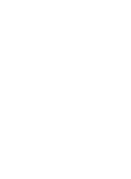
\includegraphics[width=\textwidth]{out/pdf/svg/spmv.pdf}
    \end{column}
  \end{columns}

\item<2-> accesses \ao{16 nnz} bytes and performs \ao{2 nnz} flops
  \begin{itemize}
  \item assuming elements of {\tt double} (8 bytes) and indexes of {\tt int}s (4 bytes $\times$ 2), not counting access to {\tt x} and {\tt y}
  \item details aside, it performs only \ao{\it an FMA / element}
  \end{itemize}

\item<3-> to achieve Skylake-X peak (\ao{16 DP FMAs} per core per cycle),
  a core must access \ao{16} matrix elements ($=$ \ao{256} bytes) / cycle

\item<4-> assuming 2.0GHz processor and the matrix $\gg$ cache,
  it requires the \ao{\it main memory bandwidth} of
\[ \approx 256 \mbox{ bytes} \times 2.0\mbox{ GHz} = \mbox{\aka{ 512GB/sec per core (no way!)}} \]
\end{itemize}
\end{frame}

%%%%%%%%%%%%%%%%%%%%%%%%%%%%%%%%%% 
\begin{frame}[fragile]
  \frametitle{Memory-bound algorithms (applications)}
\begin{itemize}
\item<1-> say an algorithm
  performs \ao{$C$} flops (or computation in more general) on \ao{$N$}
  bytes of data
  \begin{itemize}
  \item assume it needs to access every element of
    the $N$ bytes at least once (likely the case)
  \end{itemize}
\item<2->
  there are two obvious lower bounds on the time to complete the algorithm
  \[ T \geq \frac{C}{\mbox{the peak FLOPS}} \quad \mbox{(compute)} \]
  \[ T \geq \frac{N}{\mbox{the peak memory bandwidth}} \quad \mbox{(memory)} \]
\item<3-> often, the latter is much larger and such algorithms are called
  \ao{\it ``memory-bound''}
\item<3-> $O(N)$, $O(N \log N)$ algorithms are almost always memory bound
\end{itemize}
\end{frame}

%%%%%%%%%%%%%%%%%%%%%%%%%%%%%%%%%% 
\begin{frame}[fragile]
  \frametitle{Memory-bound algorithms (applications)}
\begin{itemize}
\item memory-bound $\iff$
  \[
    \frac{C}{\mbox{the peak FLOPS}}
    \ll \frac{N}{\mbox{the peak memory bandwidth}}
  \]
  $\iff$
  \[ \frac{C}{N} \ll \frac{\mbox{the peak FLOPS}}{\mbox{the peak memory bandwidth}} \]
  \begin{itemize}
  \item the LHS: \ao{\it arithmetic intensity} or
    \ao{\it compute intensity} of the algorithm
  \item the reciprocal of RHS: the \ao{\it byte per FLOPS}
    of the machine
  \end{itemize}

\item note that being memory-bound suggests it is
  inefficient in the processor utilization view point,
  but it is efficient in
  time-complexity sense \ao{\it (it is not necessarily a bad thing)}
\end{itemize}
\end{frame}

%%%%%%%%%%%%%%%%%%%%%%%%%%%%%%%%%% 
\begin{frame}[fragile]
\frametitle{Note: \ao{dense} matrix-vector multiply}
\begin{itemize}
\item<1-> the same argument applies even if the matrix is \ao{\it dense}
  \begin{columns}
    \begin{column}{0.05\textwidth}
    \end{column}
    \begin{column}{0.5\textwidth}
\begin{lstlisting}
for (i = 0; i < M; i++)     
  for (j = 0; j < N; j++)     
    y[i] += a[i][j] * x[j];
\end{lstlisting}
  \end{column}
    \begin{column}{0.3\textwidth}
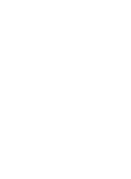
\includegraphics[width=\textwidth]{out/pdf/svg/dense_mv.pdf}
    \end{column}
  \end{columns}

\item<2-> $MN$ flops on $(MN + M + N)$ elements  
\item<3-> $\Rightarrow$ it performs only \ao{an FMA / matrix element}

\end{itemize}
\end{frame}

%%%%%%%%%%%%%%%%%%%%%%%%%%%%%%%%%% 
\begin{frame}
\frametitle{Dense matrix\ao{-matrix} multiply}
\begin{itemize}
\item<1-> the argument does \ao{\em not} apply to matrix-matrix
  multiply (we've been trying to get close to CPU peak)
  \begin{center}
  \def\svgwidth{0.5\textwidth}
  {\scriptsize \input{out/tex/svg/mm_1.pdf_tex}}
  \end{center}
  
\item<2-> for $N\times N$ square matrices,
  it performs $\ao{N^3}$ FMAs on $3 \ao{N^2}$ elements

% \item<3-> \ao{\it a single element is used by $O(N)$ FMAs},
%   so it may be possible to design a clever algorithm that
%   \begin{itemize}
%   \item brings an element into a cache, and
%   \item uses that element many times before it's evicted
%   \end{itemize}

% \item<4-> I don't mean this happens
%   automatically; \aka{\it a careful ordering of computation (blocking) is the key}
\end{itemize}
\end{frame}

%%%%%%%%%%%%%%%%% 
\begin{frame}[fragile]
  \frametitle{Why dense matrix\ao{-matrix} multiply {\it can} be efficient?}
  \begin{itemize}
  \item assume $M \sim N \sim K$
\begin{lstlisting}
for (i = 0; i < M; i++)  
  for (j = 0; j < N; j++)  
    for (k = 0; k < K; k++)  
      C(i,j) += A(i,k) * B(k,j);
\end{lstlisting}


% \item a macroscopic argument
%   \begin{itemize}
%   \item $O(N^3)$ flops on $O(N^2)$ bytes
%   \item \ao{\it if the same element does not go back and forth many times,}
%     the memory traffic is hopefully not a bottleneck
%   \end{itemize}
\item a microscopic argument
  \begin{itemize}
\item the innermost statement
\begin{lstlisting}
C(i,j) += A(i,k) * B(k,j)
\end{lstlisting}
still performs (only) \ao{1} FMA for accessing \ao{3} elements
\item but the same element (say {\tt C(i,j)}) is used many ($K$) times
  in the innermost loop
\item similarly, the same {\tt A(i,k)} is used $N$ times
\item $\Rightarrow$ after you use an element,
  \ao{\it if you reuse it many times before it is evicted from a cache
    (even a register)}, then the memory traffic is hopefully not a bottleneck
\end{itemize}
\end{itemize}

\end{frame}

%%%%%%%%%%%%%%%%% 
\begin{frame}[fragile]
\frametitle{A simple \texttt{memcpy} experiment \ldots}
\begin{itemize}
\item<1-> []
\begin{lstlisting}
double t0 = cur_time();
memcpy(a, b, nb);
double t1 = cur_time();
\end{lstlisting}
\item<2-> []
\begin{lstlisting}
$ gcc -O3 memcpy.c
$ ./a.out $((1 << 26))  # 64M long elements = 512MB
536870912 bytes copied in 0.117333 sec @\aka{\texttt{4.575611}}@ GB/sec
\end{lstlisting} %$
\item<3-> much lower than the advertised number \ldots
\end{itemize}
\end{frame}

%=================================
\section{Organization of processors, caches, and memory}
%=================================

%%%%%%%%%%%%%%%%% 
\begin{frame}
\frametitle{Cache and memory in a single-core processor}
\begin{itemize}
\item [] you almost certainly know this (\ao{\em caches} and main memory), 
  don't you? 
  
\end{itemize}
\begin{center}
\includegraphics[width=0.7\textwidth]{out/pdf/svg/diagram_single_level_cache.pdf}
\end{center}
\end{frame}

%%%%%%%%%%%%%%%%% 
\begin{frame}
\frametitle{\ldots , with multi level caches, \ldots}
\begin{itemize}
\item [] recent processors have \ao{\em multiple levels} of caches (L1, L2, \ldots)
\end{itemize}
\begin{center}
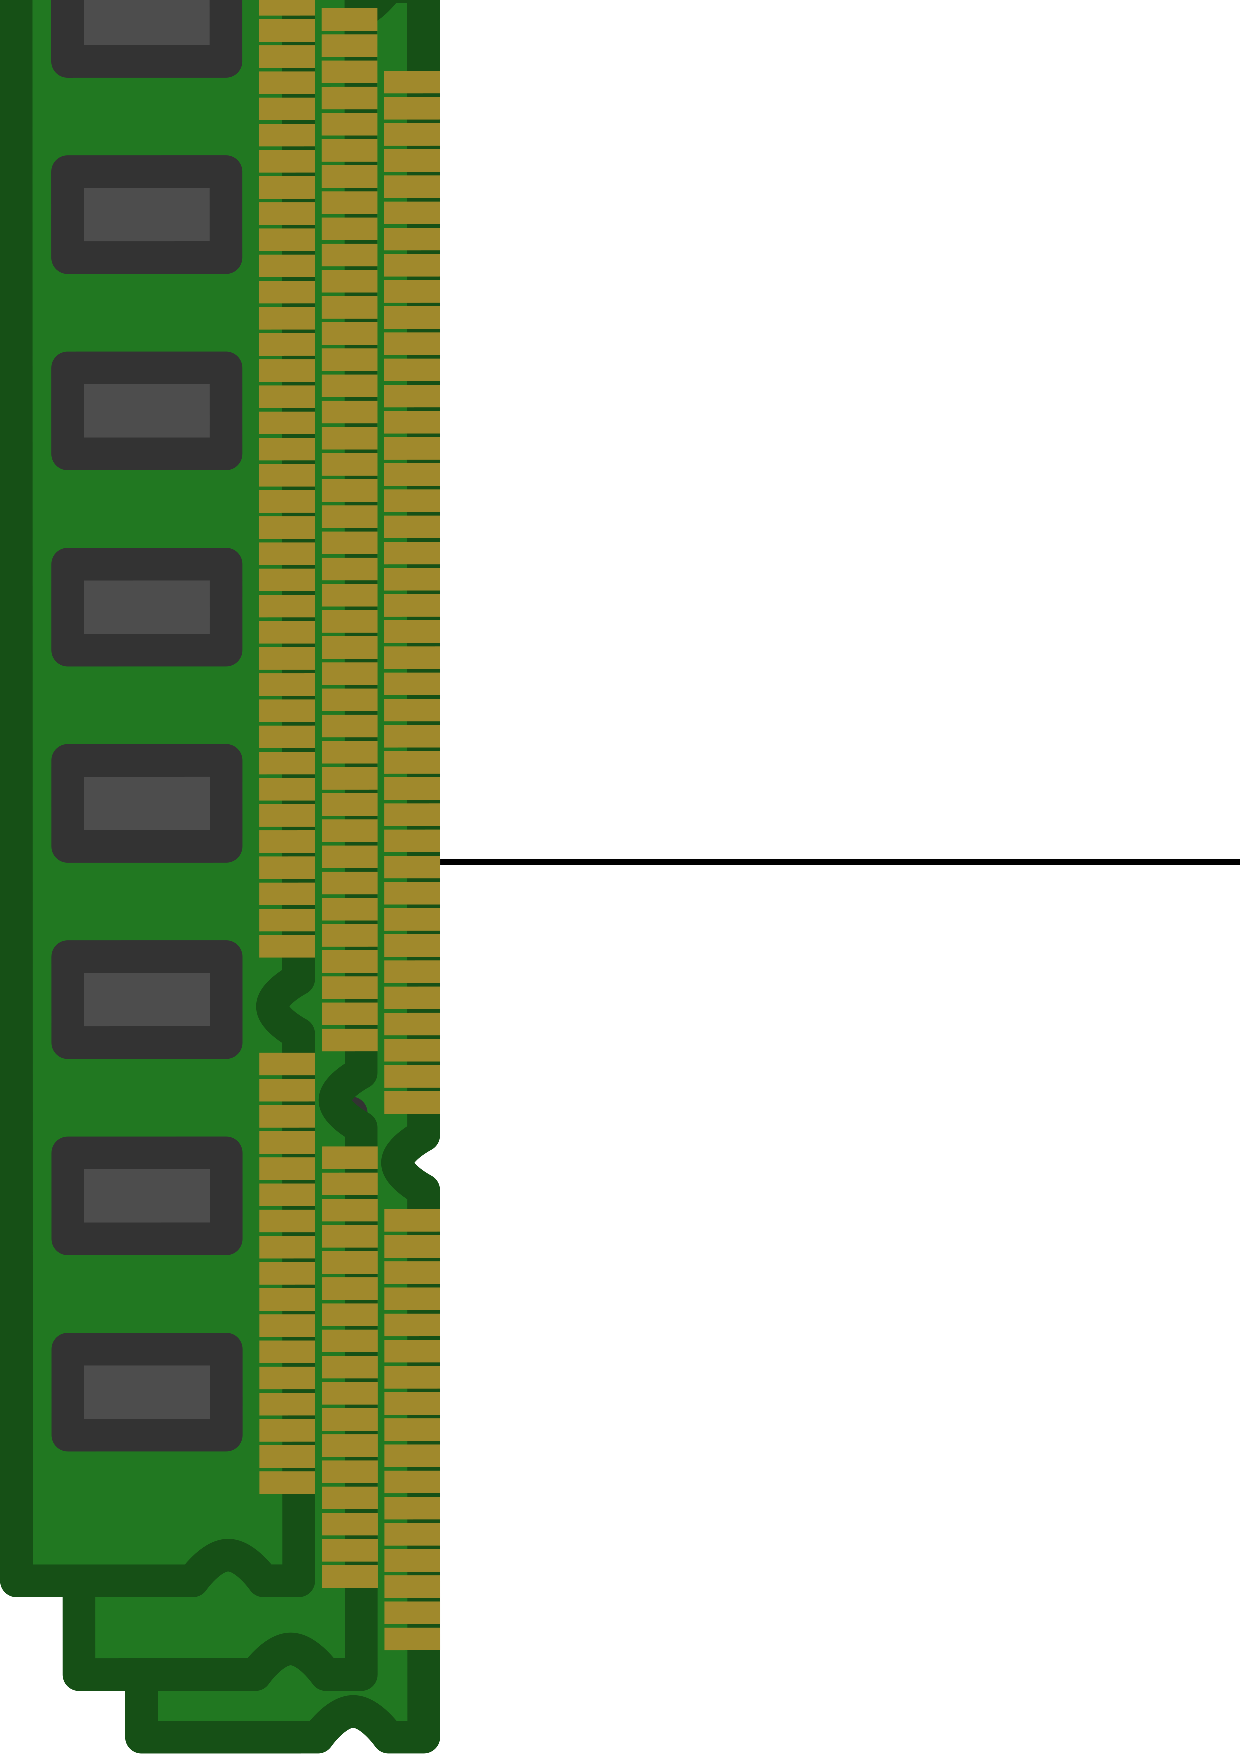
\includegraphics[width=0.7\textwidth]{out/pdf/svg/diagram_multi_level_cache.pdf}
\end{center}
\end{frame}

%%%%%%%%%%%%%%%%% 
\begin{frame}
\frametitle{\ldots , with multicores in a chip, \ldots}
\begin{itemize}
\item a single chip has several cores
\item each core has its \ao{\em private} caches (typically, L1 and L2)
\item cores in a chip share a cache (typical, L3) and main memory

\begin{center}
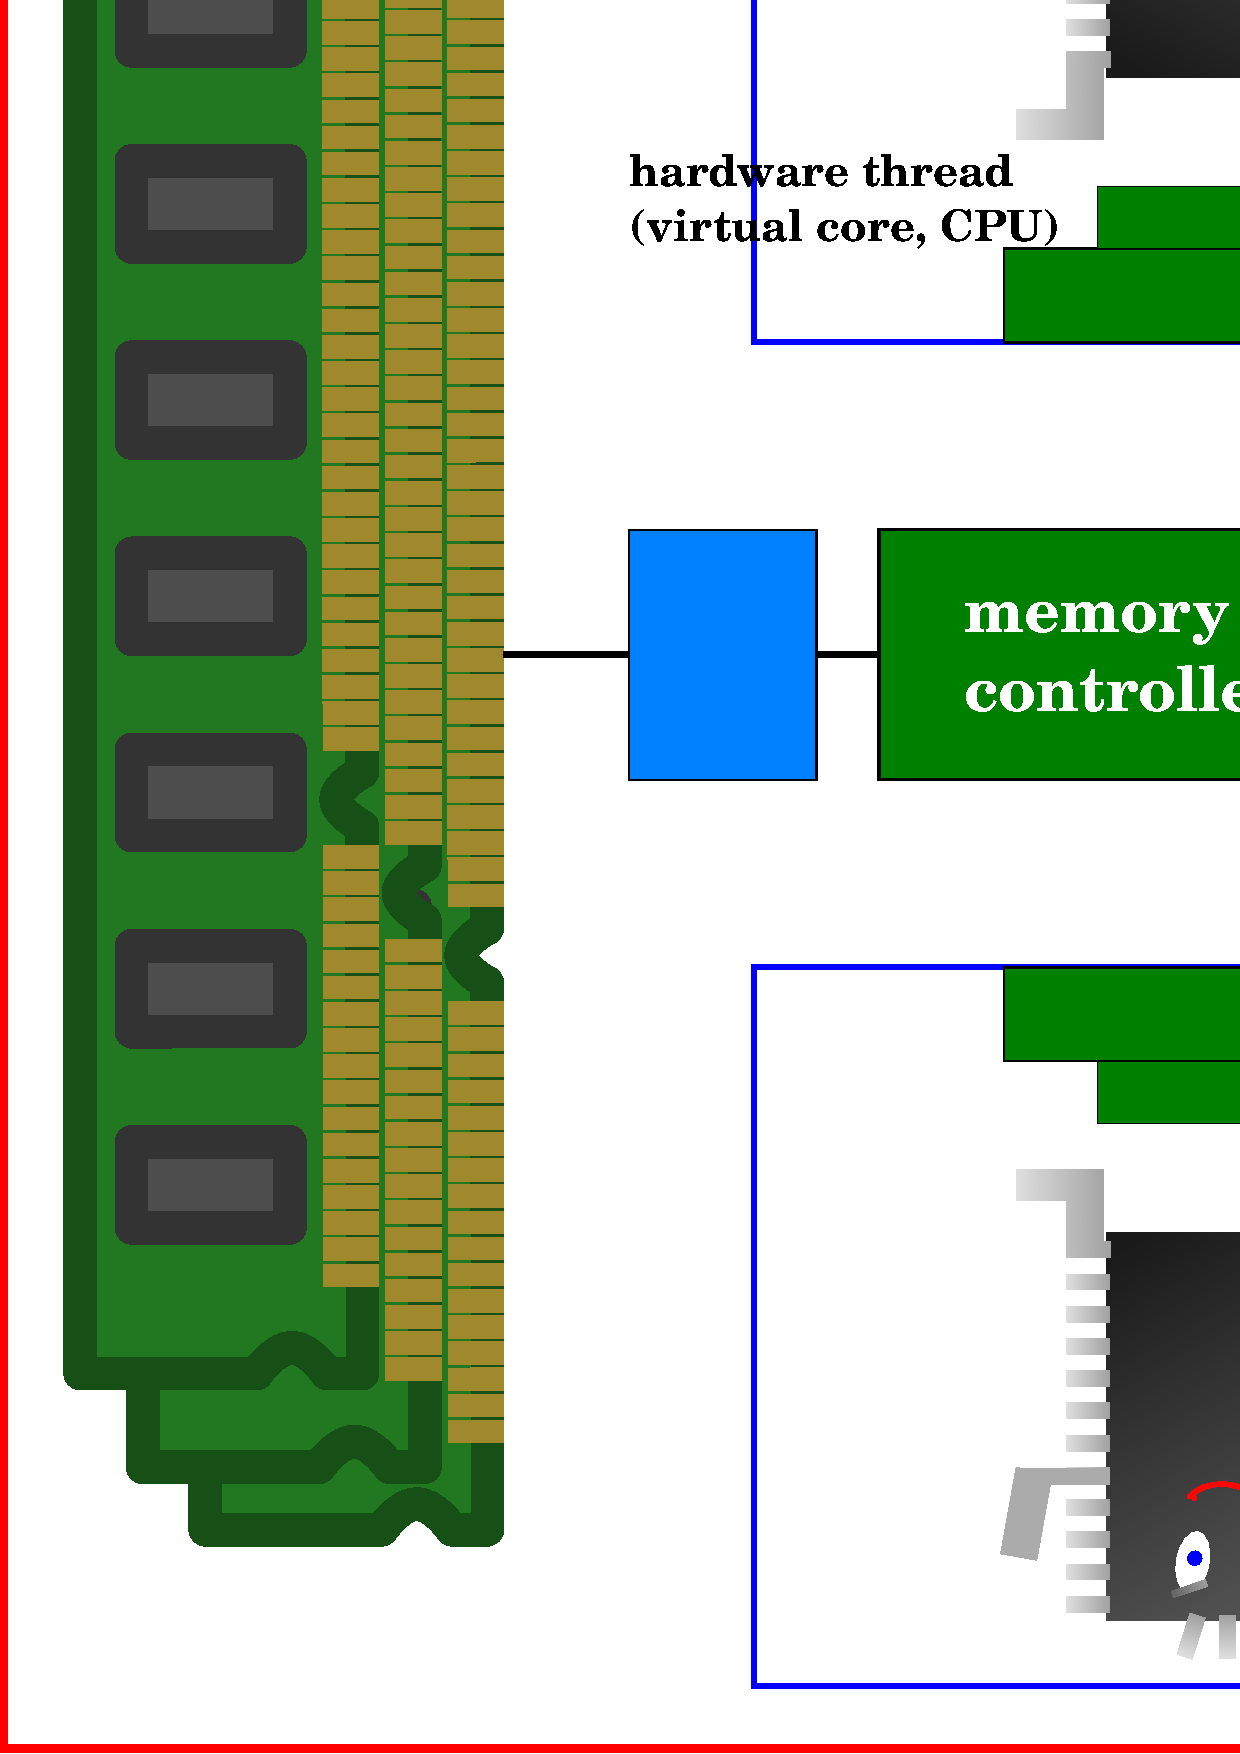
\includegraphics[width=0.6\textwidth]{out/pdf/svg/diagram_multicore.pdf}
\end{center}
\end{itemize}

\end{frame}

%%%%%%%%%%%%%%%%% 
\begin{frame}
\frametitle{\ldots , with simultaneous multithreading (SMT) in a core, \ldots}
\begin{itemize}
\item each core has two \ao{\em hardware threads}, which share
  L1/L2 caches and some or all execution units

\begin{center}
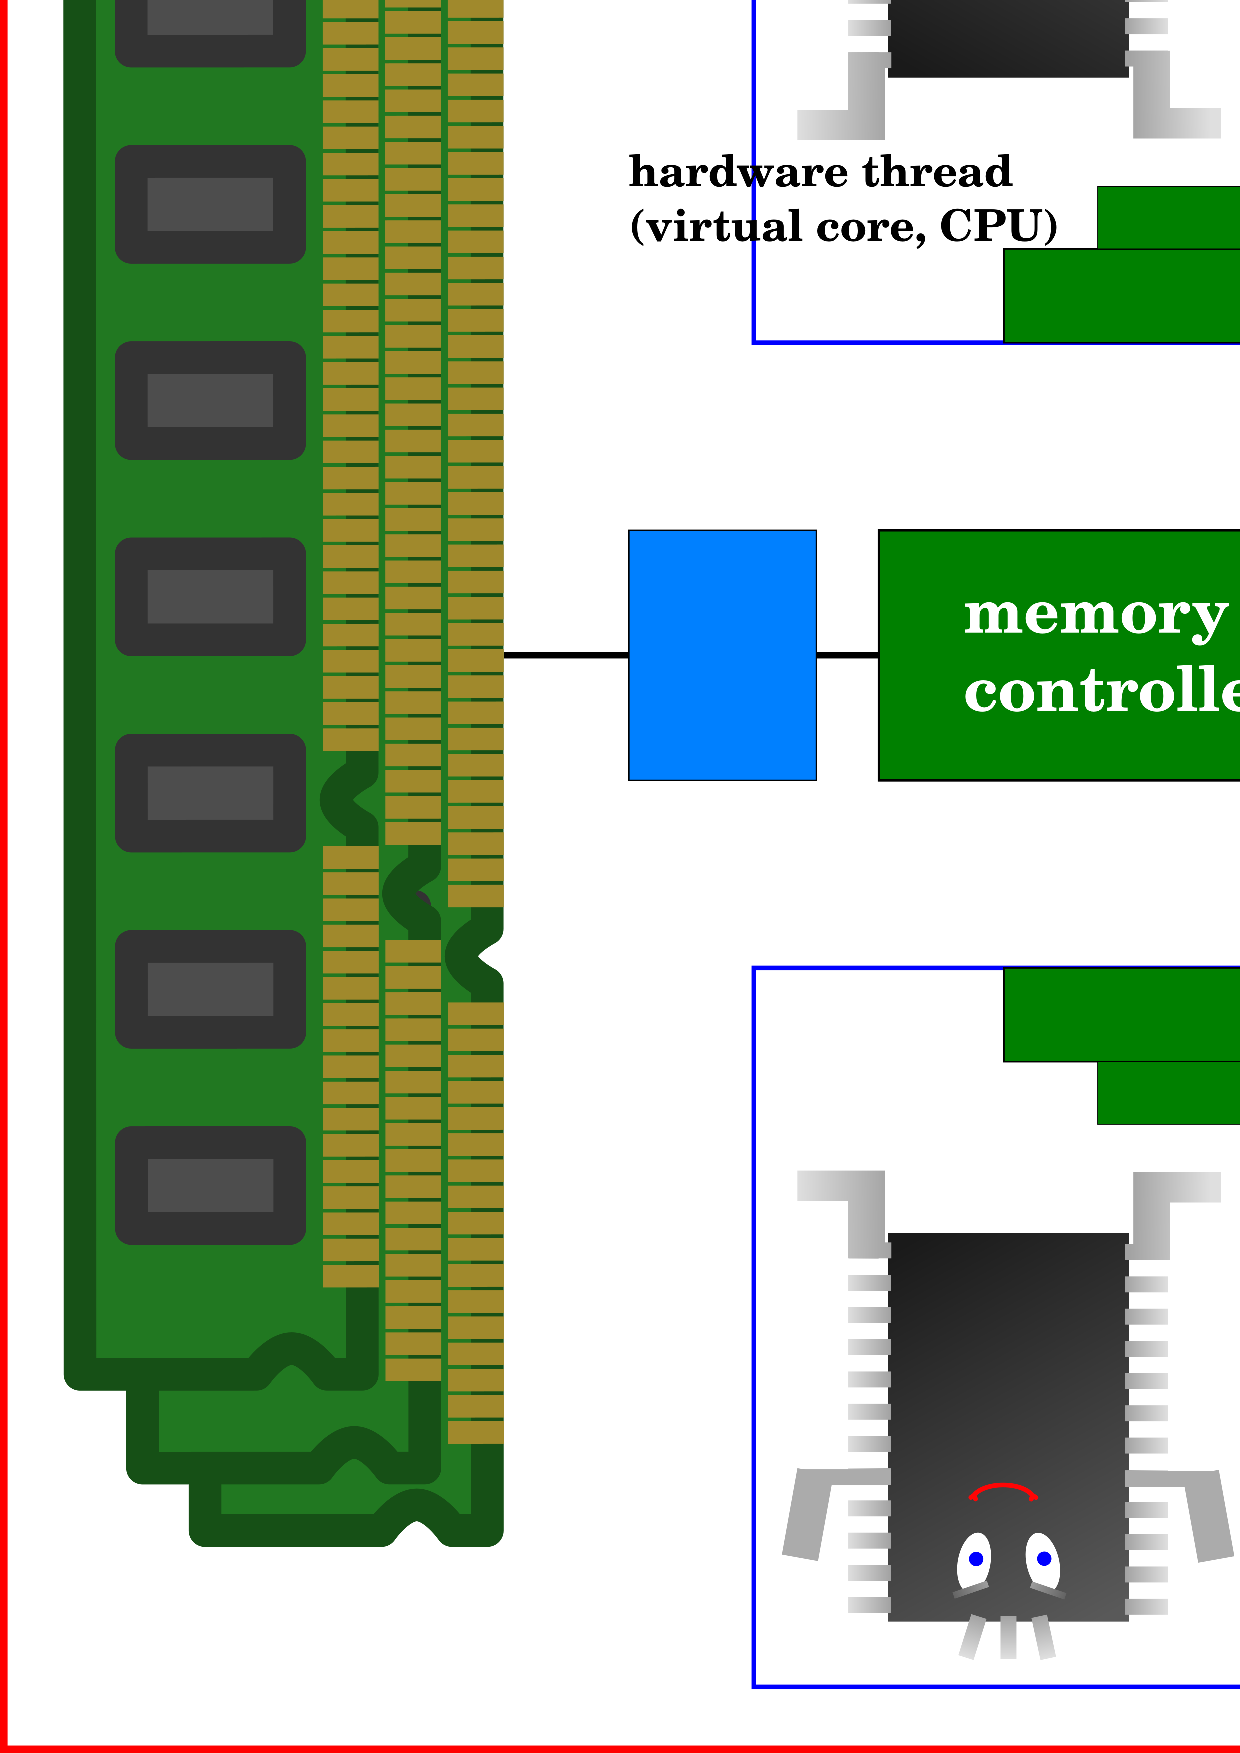
\includegraphics[width=0.6\textwidth]{out/pdf/svg/diagram_smt.pdf}
\end{center}

\end{itemize}
\end{frame}

%%%%%%%%%%%%%%%%% 
\begin{frame}
\frametitle{\ldots, and with multiple sockets per node.}
\begin{itemize}
\item each node has several chips (sockets), connected via an
interconnect (e.g., Intel QuickPath, AMD HyperTransport, etc.)
\item each socket serves a part of the entire main memory
\item each core can still access any part of the entire main memory

\begin{center}
%\def\svgwidth{0.4\textwidth}
\includegraphics[width=0.8\textwidth]{out/pdf/svg/diagram_multisocket.pdf}
\end{center}
\end{itemize}
\end{frame}


%%%%%%%%%%%%%%%%% 
\begin{frame}
\frametitle{Today's typical single compute node}
\begin{center}
\def\svgwidth{0.6\textwidth}
{\footnotesize\input{out/tex/svg/hierarchy.pdf_tex}}
\end{center}

Typical cache sizes
\begin{itemize}
\item L1 : 16KB - 64KB/core
\item L2 : 256KB - 1MB/core
\item L3 : $\sim$ 50MB/socket
\end{itemize}

\end{frame}

%=================================
%\section{Caches}
%=================================

%%%%%%%%%%%%%%%%% 
\begin{frame}
\frametitle{Cache 101}
\begin{itemize}
\item<1-> speed : 
\[ \mbox{L1} > \mbox{L2} > \mbox{L3} > \mbox{main memory} \]
\item<2-> capacity :
\[ \mbox{L1} < \mbox{L2} < \mbox{L3} < \mbox{main memory} \]
\item<3-> each cache holds a subset of data in the main memory
\[ \mbox{L1}, \mbox{L2}, \mbox{L3} \subset \mbox{main memory} \]
\item<4-> typically but not necessarily, 
  \[ \mbox{} \mbox{L1} \subset \mbox{L2} \subset \mbox{L3} \subset \mbox{main memory} \]
\item<5-> \ao{\em which subset is in caches?} 
  $\rightarrow$ cache management (replacement) policy
\end{itemize}
\end{frame}

%%%%%%%%%%%%%%%%% 
\begin{frame}
\frametitle{Cache management (replacement) policy}
\begin{itemize}

\item<1-> a cache generally holds data in \ao{\em recently accessed} 
  addresses, up to its capacity

\item<2-> this is accomplished by the \ao{LRU replacement} policy
  (or its approximation):
  \begin{itemize}
  \item every time a load/store instruction misses
    a cache, \ao{\it the least recently used data in the
      cache will be replaced}
  \end{itemize}

\item<3-> $\Rightarrow$ a (very crude) approximation; 
  data in 32KB L1 cache
\[ \approx \mbox{\ao{\em most recently accessed 32K distinct addresses}} \]

\item<4-> due to implementation constraints, real caches are slightly
  more complex
\end{itemize}
\end{frame}

%%%%%%%%%%%%%%%%% 
\begin{frame}
\frametitle{Cache organization : cache line}
\begin{columns}
\begin{column}{0.65\textwidth}
\begin{itemize}
\item<1-> a cache $=$ a set of fixed size \ao{\em lines}
  \begin{itemize}
  \item typical line size $=$ 64 bytes or 128 bytes, 
  \end{itemize}
\item<2-> a single line is the minimum unit of data transfer between levels
  (and replacement)
\end{itemize}
\end{column}

\begin{column}{0.35\textwidth}
\includegraphics[width=0.8\textwidth]{out/pdf/svg/caches_and_lines_0.pdf}

{\scriptsize a 32KB cache with 64 bytes lines
(holds most recently accessed 512 distinct blocks)}
\end{column}
\end{columns}

\vskip5mm

\only<3->{data in 32KB L1 cache (line size 64B)
\[ \approx \mbox{\ao{\em most recently accessed 512 distinct lines}} \]}
\end{frame}

%%%%%%%%%%%%%%%%%%%%%%%%%%%%%%%%%% 
\begin{frame}
\frametitle{Associativity of caches}
\begin{itemize}
\item []

\begin{columns}
  \begin{column}{0.65\textwidth}
\aka{full associative:} a block can occupy any line in the cache,
  regardless of its address
\end{column}
  \begin{column}{0.3\textwidth}
\includegraphics[width=0.9\textwidth]{out/pdf/svg/associativity_1.pdf}

  \end{column}
\end{columns}


\begin{columns}
  \begin{column}{0.65\textwidth}
\aka{direct map:} a block has only \aka{\em one} 
  designated ``seat'' (\aka{\em set}), determined by its address
\end{column}
  \begin{column}{0.3\textwidth}
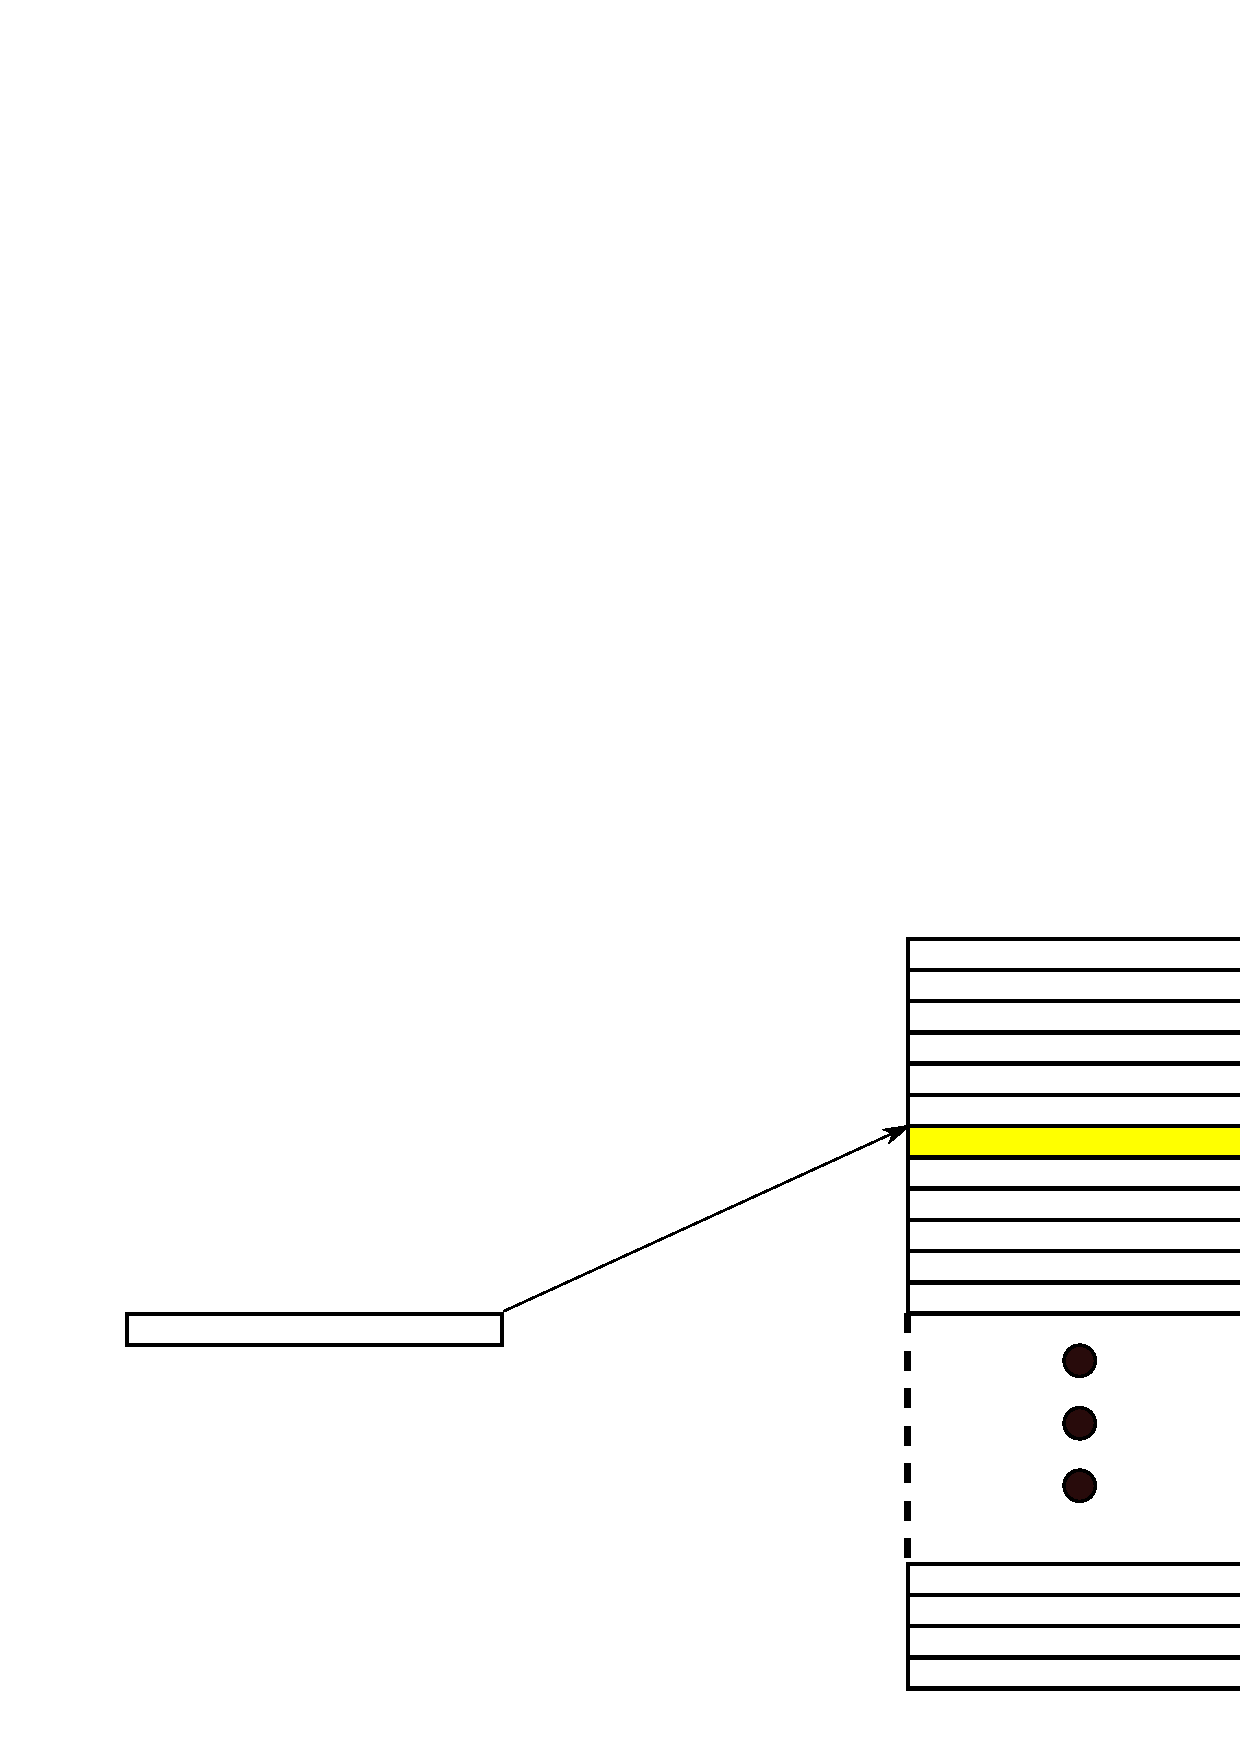
\includegraphics[width=0.9\textwidth]{out/pdf/svg/associativity_2.pdf}

  \end{column}
\end{columns}

\begin{columns}
  \begin{column}{0.65\textwidth}
\aka{$K$-way set associative:} a block has $K$
  designated ``seats'', determined by its address
  \begin{itemize}
  \item direct map $\equiv$ 1-way set associative
  \item full associative $\equiv$ $\infty$-way set associative
  \end{itemize}
\end{column}
  \begin{column}{0.3\textwidth}
\includegraphics[width=0.9\textwidth]{out/pdf/svg/associativity_3.pdf}

  \end{column}
\end{columns}
\end{itemize}
\end{frame}

%%%%%%%%%%%%%%%%%%%%%%%%%%%%%%%%%% 
\begin{frame}
\frametitle{An example cache organization}
%Ivy Bridge E5-2695 (12 cores, 2-way hyperthreading)

\begin{itemize}
\item \ao{Ice Lake Platinum 8368}

\begin{center}
\begin{tabular}{|c|c|c|c|}\hline
level & line size & capacity    & associativity \\\hline
L1    & 64B       & 48KB/core   & 12 \\  
L2    & 64B       & 512KB/core?  & 8 \\  
L3    & 64B       & 57MB/socket (38 cores) & ?? \\  \hline
\end{tabular}
\end{center}

\item Skylake-X Gold 6130

\begin{center}
\begin{tabular}{|c|c|c|c|}\hline
level & line size & capacity    & associativity \\\hline
L1    & 64B       & 32KB/core   & 8 \\  
L2    & 64B       & 1MB/core    & 16 \\  
L3    & 64B       & 22MB/socket (16 cores) & 11 \\  \hline
\end{tabular}
\end{center}

\item Ivy Bridge E5-2650L

\begin{center}
\begin{tabular}{|c|c|c|c|}\hline
level & line size & capacity    & associativity \\\hline
L1    & 64B       & 32KB/core   & 8 \\  
L2    & 64B       & 256KB/core  & 8 \\  
L3    & 64B       & 36MB/socket (8 cores) & 20 \\  \hline
\end{tabular}


\end{center}
\end{itemize}
\end{frame}

%%%%%%%%%%%%%%%%%%%%%%%%%%%%%%%%%% 
\begin{frame}
\frametitle{What you need to remember in practice about associativity}
\begin{itemize}
\item \aka{\emph{avoid having addresses used together 
      ``a-large-power-of-two'' bytes apart}}
\item corollaries:
  \begin{itemize}
  \item avoid having a matrix with a-large-power-of-two number of columns 
    \aka{(a common mistake)}
  \item avoid managing your memory by chunks of large-powers-of-two bytes
    \aka{(a common mistake)}
  \item avoid experiments only with $n = 2^p$
    \aka{(a {\it very} common mistake)}
  \end{itemize}
\item why? $\Rightarrow$ they tend to go to the same set 
  and ``conflict misses'' result
\end{itemize}
\end{frame}

%%%%%%%%%%%%%%%%%%%%%%%%%%%%%%%%%% 
\begin{frame}
\frametitle{Conflict misses}
\begin{itemize}
\item consider 8-way set associative L1 cache with 32KB (line size = 64B)
  \begin{itemize}
  \item 32KB/64B $=$ 512 ($= 2^{9}$) lines
  \item 512/8 $=$ 64 ($= 2^6$) sets
  \end{itemize}
\item $\Rightarrow$ given an address $a$, $a$[6:11] (6 bits) 
  designates the set it belongs to (indexing)
  \begin{center}
\def\svgwidth{0.8\textwidth}
{\tiny\input{out/tex/svg/addr_1.pdf_tex}}
  \end{center}

\item if two addresses $a$ and $b$ are a multiple of $2^{12}$ (4096) 
  bytes apart, they go to the same set
\end{itemize}
\end{frame}

%%%%%%%%%%%%%%%%%%%%%%%%%%%%%%%%%% 
\begin{frame}
  \frametitle{A convenient way to understand conflicts}
\begin{columns}
  \begin{column}{0.6\textwidth}
    \begin{itemize}
    \item it's convenient to think of a cache as two dimensional array of lines. e.g.
      32KB, 8-way set associative $=$ 64 (sets) $\times$ 8 (ways) array of lines
    \end{itemize}
  \end{column}

  \begin{column}{0.4\textwidth}
    \begin{center}
      \includegraphics[width=1.0\textwidth]{out/pdf/svg/conflict_1.pdf}
    \end{center}
  \end{column}

\end{columns}
\end{frame}

%%%%%%%%%%%%%%%%%%%%%%%%%%%%%%%%%% 
\begin{frame}
  \frametitle{A convenient way to understand conflicts}
\begin{columns}
  \begin{column}{0.6\textwidth}
    \begin{itemize}
    \item formula 1: 
      \[ \mbox{\aka{worst stride}} = \frac{\mbox{cache size}}{\mbox{associativity}} \mbox{ bytes} \]
      if addresses are this much apart,
      they go to the same set

      \begin{itemize}
      \item e.g., 32KB 8-way set associative
        $\Rightarrow$ the worst stride = 4096
      \end{itemize}
    \end{itemize}
  \end{column}

  \begin{column}{0.4\textwidth}
    \begin{center}
      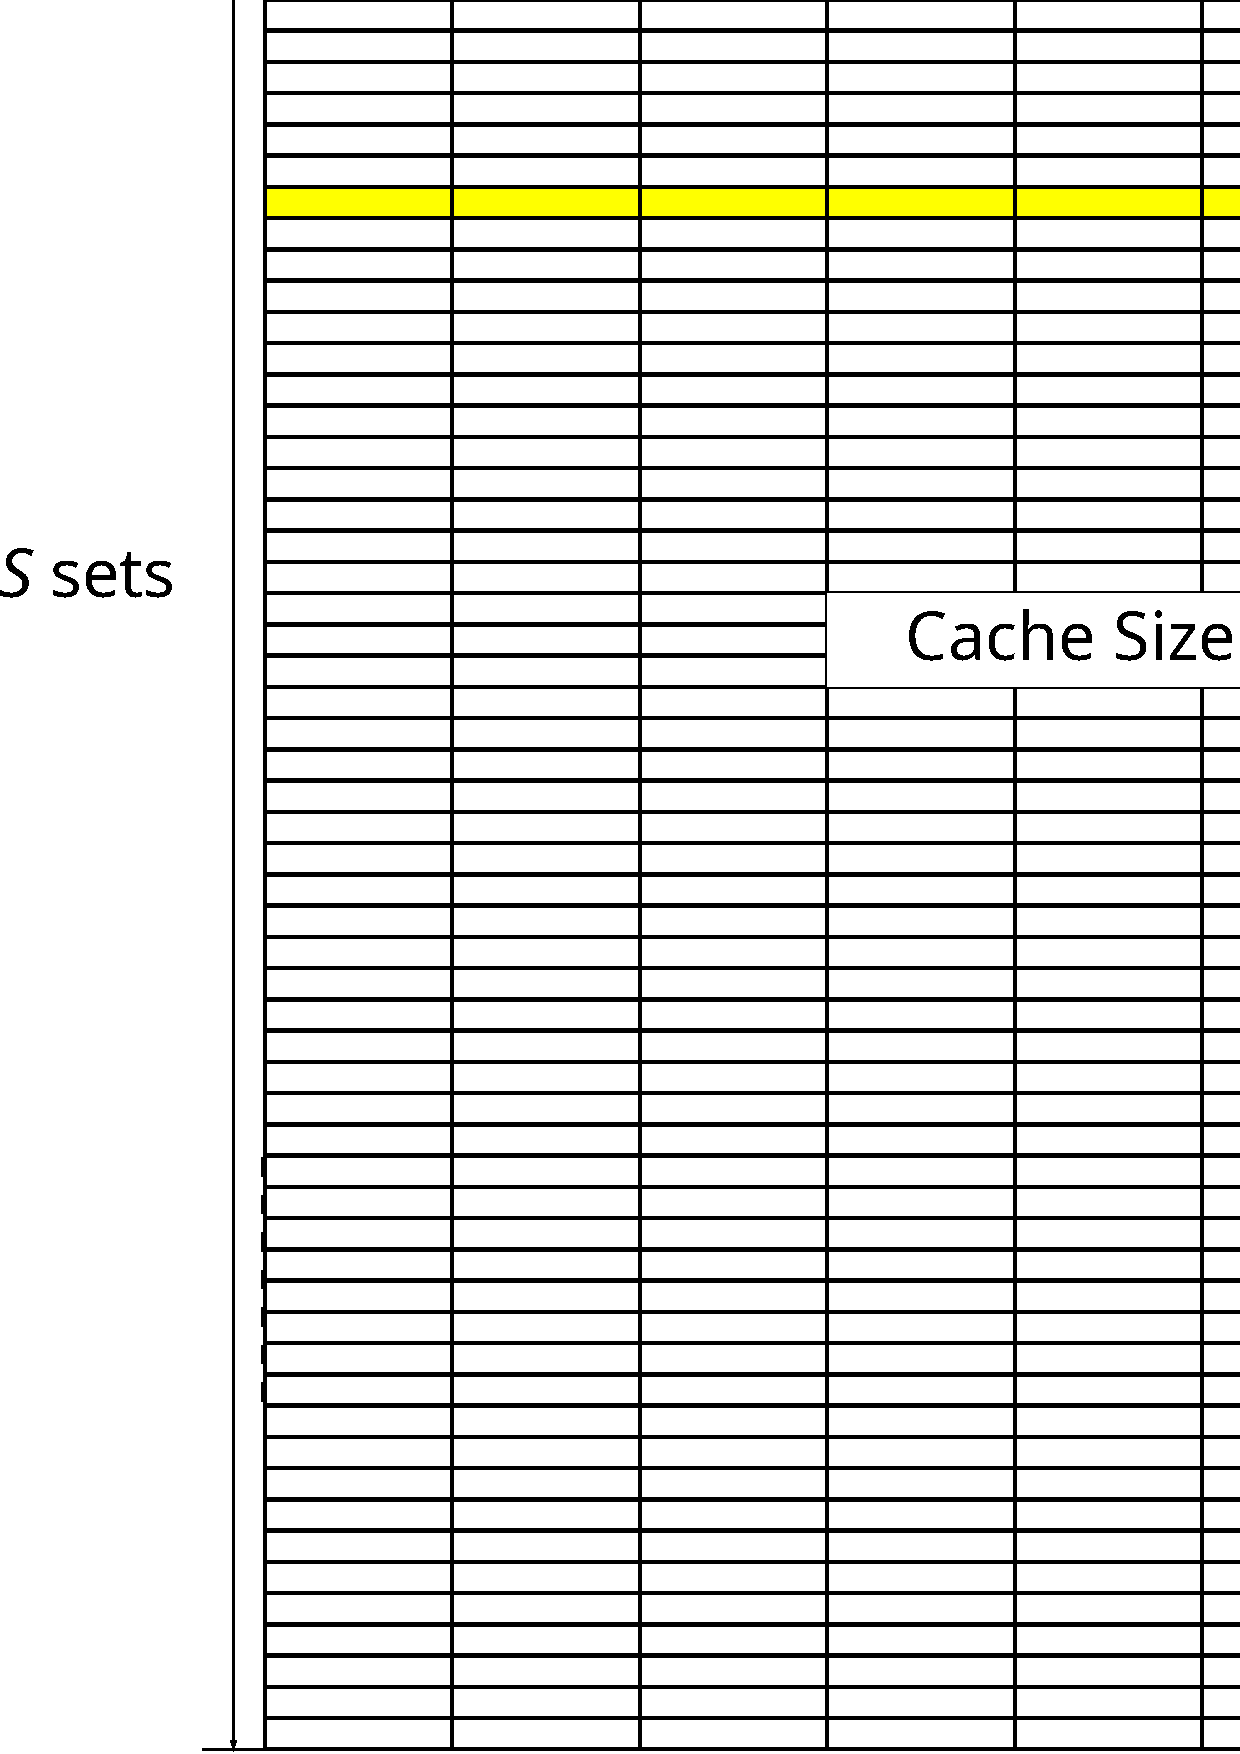
\includegraphics[width=1.0\textwidth]{out/pdf/svg/conflict_2.pdf}
    \end{center}
  \end{column}

\end{columns}
\end{frame}

%%%%%%%%%%%%%%%%%%%%%%%%%%%%%%%%%% 
\begin{frame}
  \frametitle{A convenient way to understand conflicts}
\begin{columns}
  \begin{column}{0.6\textwidth}
    \begin{itemize}
    \item lesser powers of two are significant too; continuing with
      the same setting (32KB, 8way-set assocative)
      {\tiny
      \begin{tabular}{|r|r|r|}\hline
        stride & the number of sets & utilization \\
               & they are mapped to & \\\hline
        2048   & 2  & 1/32 \\
        1024   & 4  & 1/16 \\
        512    & 8  & 1/8 \\
        256    & 16 & 1/4 \\
        128    & 32 & 1/2 \\
        64    & 64 & 1 \\
        \hline
      \end{tabular}}

  \item formula 2: you stride by
    \[ \ao{P \times \mbox{line size \quad ($P$ divides $S$)}} \]
    $\Rightarrow$ you utilize only $1/P$ of the capacity
    
  \item N.B. formula 1 is a special case, with $P = S$
    \end{itemize}
  \end{column}

  \begin{column}{0.4\textwidth}
    \begin{center}
      \includegraphics[width=1.0\textwidth]{out/pdf/svg/conflict_3.pdf}
    \end{center}
  \end{column}
\end{columns}
\end{frame}


%%%%%%%%%%%%%%%%%%%%%%%%%%%%%%%%%% 
\begin{frame}
  \frametitle{A remark about virtually-indexed vs. physically-indexed caches}
  \begin{itemize}
  \item caches typically use \ao{\it physical}
    addresses to select the set an address maps to
  \item so ``addresses'' I have been talking about are
    physical addresses, not virtual addresses you can see as pointer values

\begin{center}
\def\svgwidth{0.7\textwidth}
{\tiny\input{out/tex/svg/addr_4.pdf_tex}}
\end{center}
    
  \item since virtual $\rightarrow$ physical mapping is determined by
    the OS (based on the availability of physical memory),
    \begin{quote}
    ``two virtual addresses $2^{b}$ bytes apart''
    \end{quote}
    does \aka{\it not} necessarily imply
    \begin{quote}
      ``their physical addresses $2^{b}$ bytes apart''
    \end{quote}
  \item so what's the significance of the stories so far?
  \end{itemize}
\end{frame}

%%%%%%%%%%%%%%%%%%%%%%%%%%%%%%%%%% 
\begin{frame}
  \frametitle{A remark about virtually-indexed vs. physically-indexed caches}
  \begin{itemize}
  \item virtual $\rightarrow$ physical translation happens
    with page granularity (typically, $2^{12} = 4096$ bytes)
  \item $\rightarrow$ the last 12 bits are intact with the translation

  \begin{center}
\def\svgwidth{0.7\textwidth}
{\tiny\input{out/tex/svg/addr_3.pdf_tex}}
\end{center}

\end{itemize}
\end{frame}

%%%%%%%%%%%%%%%%%%%%%%%%%%%%%%%%%% 
\begin{frame}
  \frametitle{A remark about virtually-indexed vs. physically-indexed caches}
  \begin{itemize}
  \item therefore,
    \begin{quote}
      ``two \ao{\em virtual} addresses $2^{b}$ bytes apart''
      $\rightarrow$
      ``their \ao{\em physical} addresses $2^{b}$ bytes apart''
    \end{quote}
    \ao{\it for up to page size ($2^b \leq$ page size)}
  \item $\rightarrow$ the formula 2 is valid
    for strides up to page size

    \begin{columns}
      \begin{column}{0.3\textwidth}
    {\scriptsize
      \begin{tabular}{|r|r|}\hline
        stride & utilization \\\hline
        4096   & 1/64 \\
        2048   & 1/32 \\
        1024   & 1/16 \\
        512    & 1/8 \\
        256    & 1/4 \\
        128    & 1/2 \\
        64     & 1 \\
        \hline
      \end{tabular}}
  \end{column}
  \begin{column}{0.7\textwidth}
\def\svgwidth{1.0\textwidth}
{\tiny\input{out/tex/svg/addr_3.pdf_tex}}
  \end{column}  
    \end{columns}
  \end{itemize}
\end{frame}

%%%%%%%%%%%%%%%%%%%%%%%%%%%%%%%%%% 
\begin{frame}
  \frametitle{Remarks applied to different cache levels}
  \begin{columns}
    \begin{column}{0.7\textwidth}
  \begin{itemize}
  \item small caches that use only the last 12 bits to index the set
    make no difference between virtually- and physically-indexed caches
    
  \item for larger caches,
    the utilization will similarly drop up to stride $=$ 4096,
    after which it will stay around 1/64
  \end{itemize}
    \end{column}
    \begin{column}{0.3\textwidth}
    {\scriptsize
      \begin{tabular}{|r|r|}\hline
        stride & utilization \\\hline
        \ldots & $\sim$ 1/64 \\
        16384  & $\sim$ 1/64 \\
        8192   & $\sim$ 1/64 \\
        4096   & 1/64 \\
        2048   & 1/32 \\
        1024   & 1/16 \\
        512    & 1/8 \\
        256    & 1/4 \\
        128    & 1/2 \\
        64     & 1 \\
        \hline
      \end{tabular}}
    \end{column}
  \end{columns}

  \begin{itemize}
  \item L1 (32KB/8-way) vs. L2 (256KB/8-way)
\begin{center}
\def\svgwidth{0.6\textwidth}
{\tiny\input{out/tex/svg/addr_2.pdf_tex}}
\vskip5mm
\def\svgwidth{0.6\textwidth}
{\tiny\input{out/tex/svg/addr_3.pdf_tex}}
\end{center}
\end{itemize}

\end{frame}


%%%%%%%%%%%%%%%%%%%%%%%%%%%%%%%%%% 
\begin{frame}[fragile]
\frametitle{Avoiding conflict misses}
\begin{itemize}
\item e.g., if you have a matrix:
\begin{lstlisting}
float a[100][1024];
\end{lstlisting}
then \texttt{a[i][j]} and \texttt{a[i+1][j]} go to the same set in L1 cache; 
\item $\Rightarrow$
scanning a column of such a matrix will experience 
almost 100\% cache miss
\item avoid it by:
\begin{lstlisting}
float a[100][1024@\ao{\texttt{+16}}@];
\end{lstlisting}
\end{itemize}
\end{frame}

%%%%%%%%%%%%%%%%%%%%%%%%%%%%%%%%%% 
\begin{frame}
\frametitle{What are in the cache?}

\begin{itemize}
\item<1-> consider a cache of
  \begin{itemize}
  \item capacity $= \ao{C}$ bytes
  \item line size $= \ao{Z}$ bytes
  \item associativity $=$ \ao{$K$}
  \end{itemize}
\item<2-> \ao{approximation 0.0 (only consider $C$; $\equiv Z = 1, K = \infty$):} 
\[ \mbox{Cache} \approx \mbox{most recently accessed $C$ distinct addresses} \]

\item<3-> \ao{approximation 1.0 (only consider $C$ and $Z$; $K = \infty$):} 
  \[ \mbox{Cache} \approx \mbox{most recently accessed $C/Z$ distinct lines} \]
  \iffalse
more pragmatically, if you typically access data larger than cache line granularity
(i.e., when you touch an element, you almost certainly touch the surrounding $Z$ bytes), 
forget $Z$; otherwise cache $\approx$
\mbox{most recently accessed $C/Z$ elements}
\fi

\item<4-> \ao{approximation 2.0 (consider associativity too):}
  \begin{itemize}
  \item depending on the stride of the addresses you use,
    reason about the utilization (effective size) of the cache
  \item in practice, avoid strides of ``line size $\times 2^b$''
\end{itemize}
\end{itemize}
\end{frame}


% =================================
\section{So how costly is it to access data?}
% =================================

%%%%%%%%%%%%%%%%%%%%%%%%%%%%%%%%%% 
\begin{frame}
  \frametitle{Assessing the cost of data access}
  \begin{itemize}
  \item we like to obtain cost to access data in each level
    of the caches as well as main memory

  \item \ao{latency:} time until the result of a
    load instruction becomes available

  \item \ao{bandwidth:} the maximum amount of data per unit time that
    can be transferred between the layer in question
    to CPU (registers)

  \end{itemize}
\end{frame}

% =================================
\subsection{Latency}
% =================================

%%%%%%%%%%%%%%%%%%%%%%%%%%%%%%%%%% 
\begin{frame}[fragile]
  \frametitle{How to measure a latency?}
  \begin{itemize}

  \item<1-> prepare an array of $N$ records and access
    them repeatedly

  \item<2-> to measure the {\em latency},
    make sure $N$ load instructions \ao{\em make a chain of dependencies} (link list traversal)

\begin{lstlisting}
for (@$N$@ times) {
  p = p->next;
}
\end{lstlisting}

\item<3-> make sure {\tt p->next} links all the
  elements in a random order (the reason becomes clear later)

\begin{center}
\def\svgwidth{0.6\textwidth}
{\scriptsize \input{out/tex/svg/measure_latency.pdf_tex}}
\end{center}
\end{itemize}
\end{frame}


%%%%%%%%%%%%%%%%%%%%%%%%%%%%%%%%%% 
\begin{frame}[fragile]
\frametitle{Data size vs. latency}
\begin{itemize}
\item main memory is local to the accessing thread
\begin{lstlisting}
$ numactl --cpunodebind 0 --interleave 0 ./mem
$ numactl -N 0 -i 0 ./mem   # abbreviation
\end{lstlisting}

\begin{columns}
\begin{column}{0.75\textwidth}
%{\scriptsize\input{out/tex/data/mem/latency_local_0.tex}}
{\scriptsize% GNUPLOT: LaTeX picture with Postscript
\begingroup
  \makeatletter
  \providecommand\color[2][]{%
    \GenericError{(gnuplot) \space\space\space\@spaces}{%
      Package color not loaded in conjunction with
      terminal option `colourtext'%
    }{See the gnuplot documentation for explanation.%
    }{Either use 'blacktext' in gnuplot or load the package
      color.sty in LaTeX.}%
    \renewcommand\color[2][]{}%
  }%
  \providecommand\includegraphics[2][]{%
    \GenericError{(gnuplot) \space\space\space\@spaces}{%
      Package graphicx or graphics not loaded%
    }{See the gnuplot documentation for explanation.%
    }{The gnuplot epslatex terminal needs graphicx.sty or graphics.sty.}%
    \renewcommand\includegraphics[2][]{}%
  }%
  \providecommand\rotatebox[2]{#2}%
  \@ifundefined{ifGPcolor}{%
    \newif\ifGPcolor
    \GPcolortrue
  }{}%
  \@ifundefined{ifGPblacktext}{%
    \newif\ifGPblacktext
    \GPblacktexttrue
  }{}%
  % define a \g@addto@macro without @ in the name:
  \let\gplgaddtomacro\g@addto@macro
  % define empty templates for all commands taking text:
  \gdef\gplbacktext{}%
  \gdef\gplfronttext{}%
  \makeatother
  \ifGPblacktext
    % no textcolor at all
    \def\colorrgb#1{}%
    \def\colorgray#1{}%
  \else
    % gray or color?
    \ifGPcolor
      \def\colorrgb#1{\color[rgb]{#1}}%
      \def\colorgray#1{\color[gray]{#1}}%
      \expandafter\def\csname LTw\endcsname{\color{white}}%
      \expandafter\def\csname LTb\endcsname{\color{black}}%
      \expandafter\def\csname LTa\endcsname{\color{black}}%
      \expandafter\def\csname LT0\endcsname{\color[rgb]{1,0,0}}%
      \expandafter\def\csname LT1\endcsname{\color[rgb]{0,1,0}}%
      \expandafter\def\csname LT2\endcsname{\color[rgb]{0,0,1}}%
      \expandafter\def\csname LT3\endcsname{\color[rgb]{1,0,1}}%
      \expandafter\def\csname LT4\endcsname{\color[rgb]{0,1,1}}%
      \expandafter\def\csname LT5\endcsname{\color[rgb]{1,1,0}}%
      \expandafter\def\csname LT6\endcsname{\color[rgb]{0,0,0}}%
      \expandafter\def\csname LT7\endcsname{\color[rgb]{1,0.3,0}}%
      \expandafter\def\csname LT8\endcsname{\color[rgb]{0.5,0.5,0.5}}%
    \else
      % gray
      \def\colorrgb#1{\color{black}}%
      \def\colorgray#1{\color[gray]{#1}}%
      \expandafter\def\csname LTw\endcsname{\color{white}}%
      \expandafter\def\csname LTb\endcsname{\color{black}}%
      \expandafter\def\csname LTa\endcsname{\color{black}}%
      \expandafter\def\csname LT0\endcsname{\color{black}}%
      \expandafter\def\csname LT1\endcsname{\color{black}}%
      \expandafter\def\csname LT2\endcsname{\color{black}}%
      \expandafter\def\csname LT3\endcsname{\color{black}}%
      \expandafter\def\csname LT4\endcsname{\color{black}}%
      \expandafter\def\csname LT5\endcsname{\color{black}}%
      \expandafter\def\csname LT6\endcsname{\color{black}}%
      \expandafter\def\csname LT7\endcsname{\color{black}}%
      \expandafter\def\csname LT8\endcsname{\color{black}}%
    \fi
  \fi
    \setlength{\unitlength}{0.0500bp}%
    \ifx\gptboxheight\undefined%
      \newlength{\gptboxheight}%
      \newlength{\gptboxwidth}%
      \newsavebox{\gptboxtext}%
    \fi%
    \setlength{\fboxrule}{0.5pt}%
    \setlength{\fboxsep}{1pt}%
    \definecolor{tbcol}{rgb}{1,1,1}%
\begin{picture}(5102.00,3118.00)%
    \gplgaddtomacro\gplbacktext{%
      \csname LTb\endcsname%%
      \put(592,713){\makebox(0,0)[r]{\strut{}$0$}}%
      \put(592,927){\makebox(0,0)[r]{\strut{}$50$}}%
      \put(592,1141){\makebox(0,0)[r]{\strut{}$100$}}%
      \put(592,1354){\makebox(0,0)[r]{\strut{}$150$}}%
      \put(592,1568){\makebox(0,0)[r]{\strut{}$200$}}%
      \put(592,1782){\makebox(0,0)[r]{\strut{}$250$}}%
      \put(592,1996){\makebox(0,0)[r]{\strut{}$300$}}%
      \put(592,2209){\makebox(0,0)[r]{\strut{}$350$}}%
      \put(592,2423){\makebox(0,0)[r]{\strut{}$400$}}%
      \put(592,2637){\makebox(0,0)[r]{\strut{}$450$}}%
      \put(688,617){\rotatebox{-20.00}{\makebox(0,0)[l]{\strut{}$4096$}}}%
      \put(1146,617){\rotatebox{-20.00}{\makebox(0,0)[l]{\strut{}$16384$}}}%
      \put(1605,617){\rotatebox{-20.00}{\makebox(0,0)[l]{\strut{}$65536$}}}%
      \put(2063,617){\rotatebox{-20.00}{\makebox(0,0)[l]{\strut{}$262144$}}}%
      \put(2521,617){\rotatebox{-20.00}{\makebox(0,0)[l]{\strut{}$1.04858\times10^{6}$}}}%
      \put(2980,617){\rotatebox{-20.00}{\makebox(0,0)[l]{\strut{}$4.1943\times10^{6}$}}}%
      \put(3438,617){\rotatebox{-20.00}{\makebox(0,0)[l]{\strut{}$1.67772\times10^{7}$}}}%
      \put(3896,617){\rotatebox{-20.00}{\makebox(0,0)[l]{\strut{}$6.71089\times10^{7}$}}}%
      \put(4355,617){\rotatebox{-20.00}{\makebox(0,0)[l]{\strut{}$2.68435\times10^{8}$}}}%
      \put(4813,617){\rotatebox{-20.00}{\makebox(0,0)[l]{\strut{}$1.07374\times10^{9}$}}}%
    }%
    \gplgaddtomacro\gplfronttext{%
      \csname LTb\endcsname%%
      \put(1264,2494){\makebox(0,0)[r]{\strut{}local}}%
      \csname LTb\endcsname%%
      \put(152,1675){\rotatebox{-270.00}{\makebox(0,0){\strut{}latency/load (CPU cycles)}}}%
      \put(2750,112){\makebox(0,0){\strut{}size of the region (bytes)}}%
      \put(2750,2877){\makebox(0,0){\strut{}latency per load in a random list traversal [0,1073741824]}}%
    }%
    \gplbacktext
    \put(0,0){\includegraphics[width={255.10bp},height={155.90bp}]{out/tex/data/08mem//latency_local_big_0_1073741824}}%
    \gplfronttext
  \end{picture}%
\endgroup
}
%out/tex/data/08mem/latency\_local\_big\_0\_1073741824.tex
\end{column}
\begin{column}{0.25\textwidth}
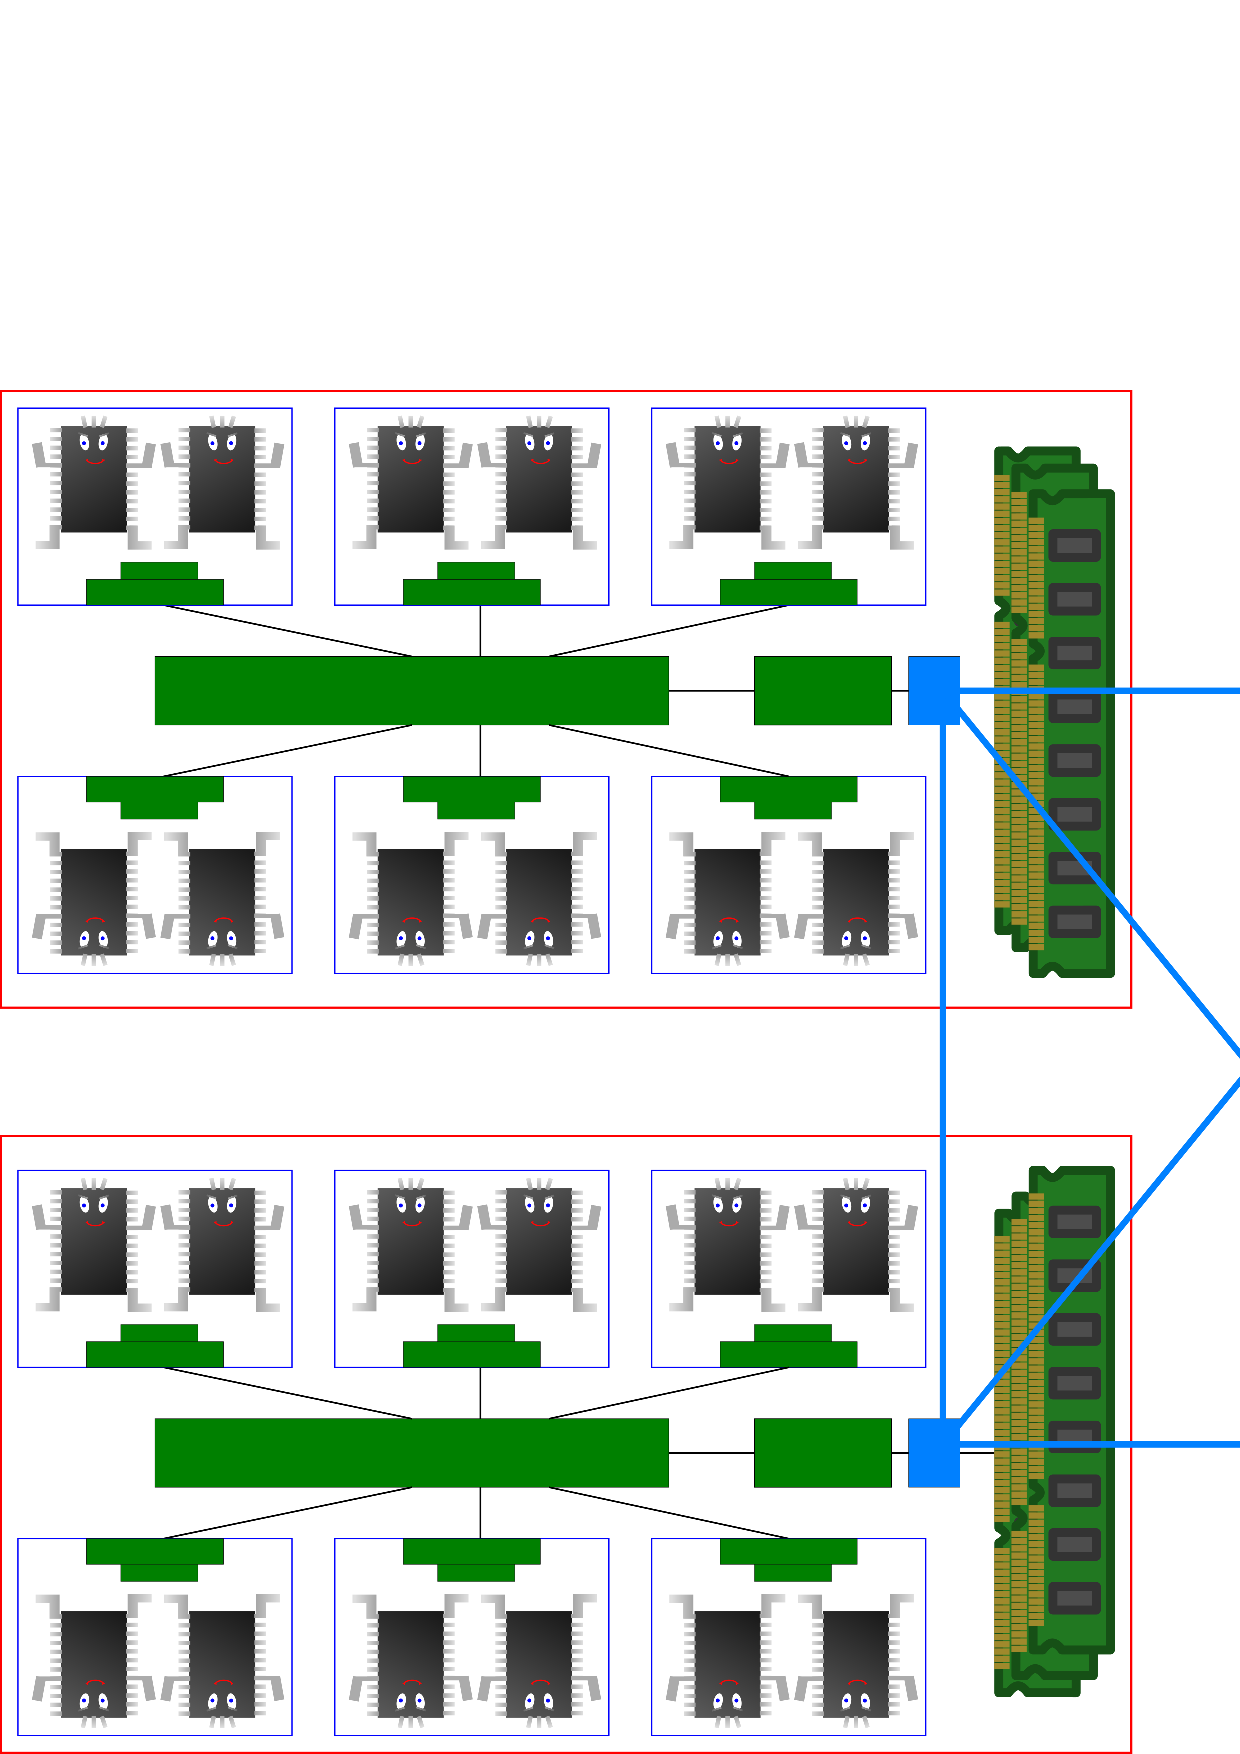
\includegraphics[width=\textwidth]{out/pdf/svg/diagram_multisocket_local.pdf}
\end{column}
\end{columns}
\end{itemize}
\end{frame}


%%%%%%%%%%%%%%%%%%%%%%%%%%%%%%%%%% 
\begin{frame}
\frametitle{How long are latencies}
\begin{itemize}
\item heavily depends on in which level of the cache data fit
\item environment: Skylake-X Xeon Gold 6130 (32KB/1MB/22MB)
\end{itemize}

\begin{columns}
  \begin{column}{0.4\textwidth}
{\scriptsize
\begin{tabular}{|r|r|r|r|}\hline
size         & level & latency  & latency \\
             &       & (cycles) & (ns)    \\\hline
  12,736     & L1    & 4.004    & 1.31     \\
 103,616     & L2    & 13.80    & 4.16     \\
 2,964,928   & L3    & 77.40    & 24.24    \\
 301,307,584 & main  & 377.60   & 115.45   \\\hline
\end{tabular}
}
\end{column}
\begin{column}{0.05\textwidth}
\end{column}
\begin{column}{0.55\textwidth}
\begin{center}
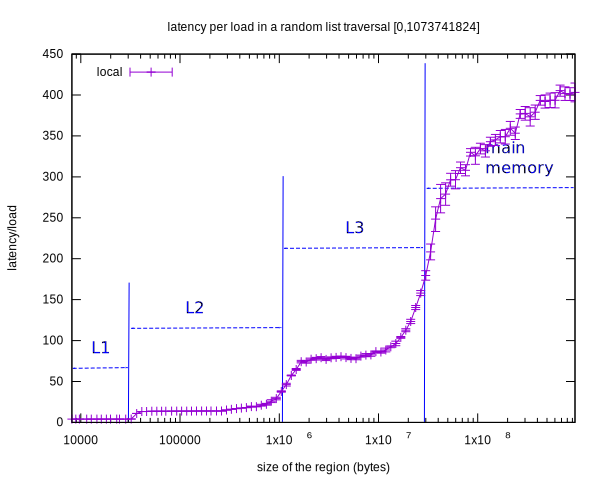
\includegraphics[width=\textwidth]{out/pdf/svg/latency_cliff.pdf}
\end{center}
\end{column}
\end{columns}
\end{frame}

%%%%%%%%%%%%%%%%%%%%%%%%%%%%%%%%%% 
\begin{frame}
\frametitle{A remark about replacement policy}
\begin{itemize}
\item if a cache stricly follows the LRU replacement policy, 
  once data overflow the cache, repeated access to the data
  will quickly become \ao{\emph{almost-always-miss}}

\item the ``cliffs'' in the experimental data
  look gentler than the theory would suggest

\begin{columns}
  \begin{column}{0.5\textwidth}
\def\svgwidth{\textwidth}
\only<1>{\tiny\input{out/tex/svg/lru_behavior_1.pdf_tex}}%
\only<2>{\tiny\input{out/tex/svg/lru_behavior_2.pdf_tex}}%
\only<3>{\tiny\input{out/tex/svg/lru_behavior_3.pdf_tex}}
  \end{column}  
  \begin{column}{0.5\textwidth}
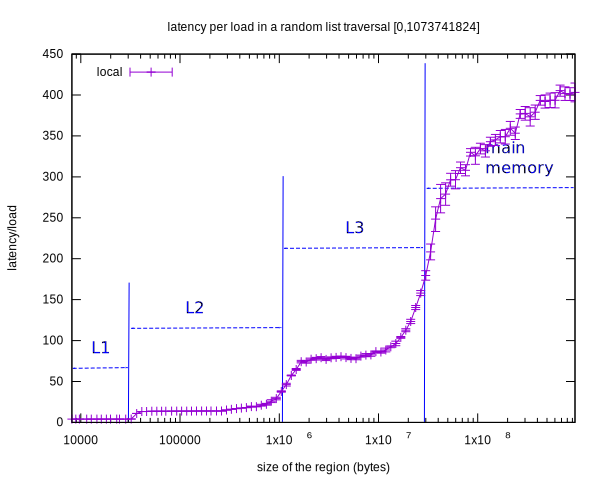
\includegraphics[width=0.9\textwidth]{out/pdf/svg/latency_cliff.pdf}
  \end{column}
\end{columns}
\end{itemize}
\end{frame}


%%%%%%%%%%%%%%%%%%%%%%%%%%%%%%%%%% 
\begin{frame}
\frametitle{A remark about replacement policy}
\begin{itemize}

\item part of the gap is due to virtual $\rightarrow$ physical
  address translation

\item another factor, especially for L3 cache, will be
  a recent replacement policy for cyclic accesses
(c.f. \url{http://blog.stuffedcow.net/2013/01/ivb-cache-replacement/})

\begin{columns}
  \begin{column}{0.5\textwidth}
\def\svgwidth{\textwidth}
{\tiny\input{out/tex/svg/lru_behavior_3.pdf_tex}}
  \end{column}  
  \begin{column}{0.5\textwidth}
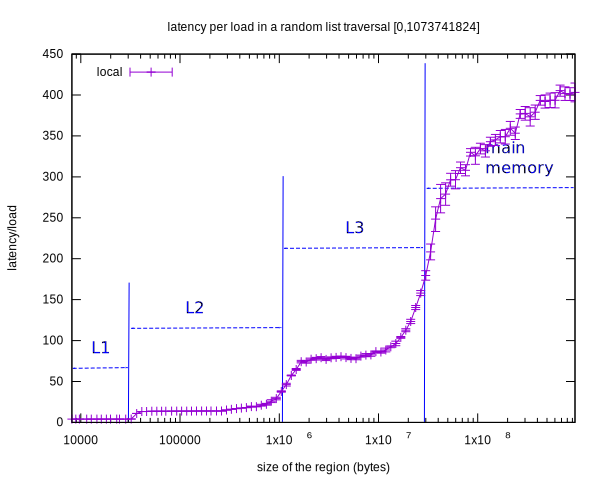
\includegraphics[width=0.9\textwidth]{out/pdf/svg/latency_cliff.pdf}
  \end{column}
\end{columns}
\end{itemize}
\end{frame}

%%%%%%%%%%%%%%%%%%%%%%%%%%%%%%%%%% 
\begin{frame}[fragile]
\frametitle{Latency to a remote main memory}
\begin{itemize}
\item make main memory remote to the accessing thread
\begin{lstlisting}
$ numactl -N 0 -i 1 ./mem
\end{lstlisting} %$
\begin{columns}
\begin{column}{0.75\textwidth}
%{\scriptsize\input{out/tex/data/mem/latency_local_remote_0.tex}}
{\scriptsize\input{out/tex/data/08mem/latency_local_remote_big_0_1073741824.tex}}
%out/tex/data/08mem/latency\_local\_remote\_big\_0\_1073741824.tex
\end{column}
\begin{column}{0.25\textwidth}
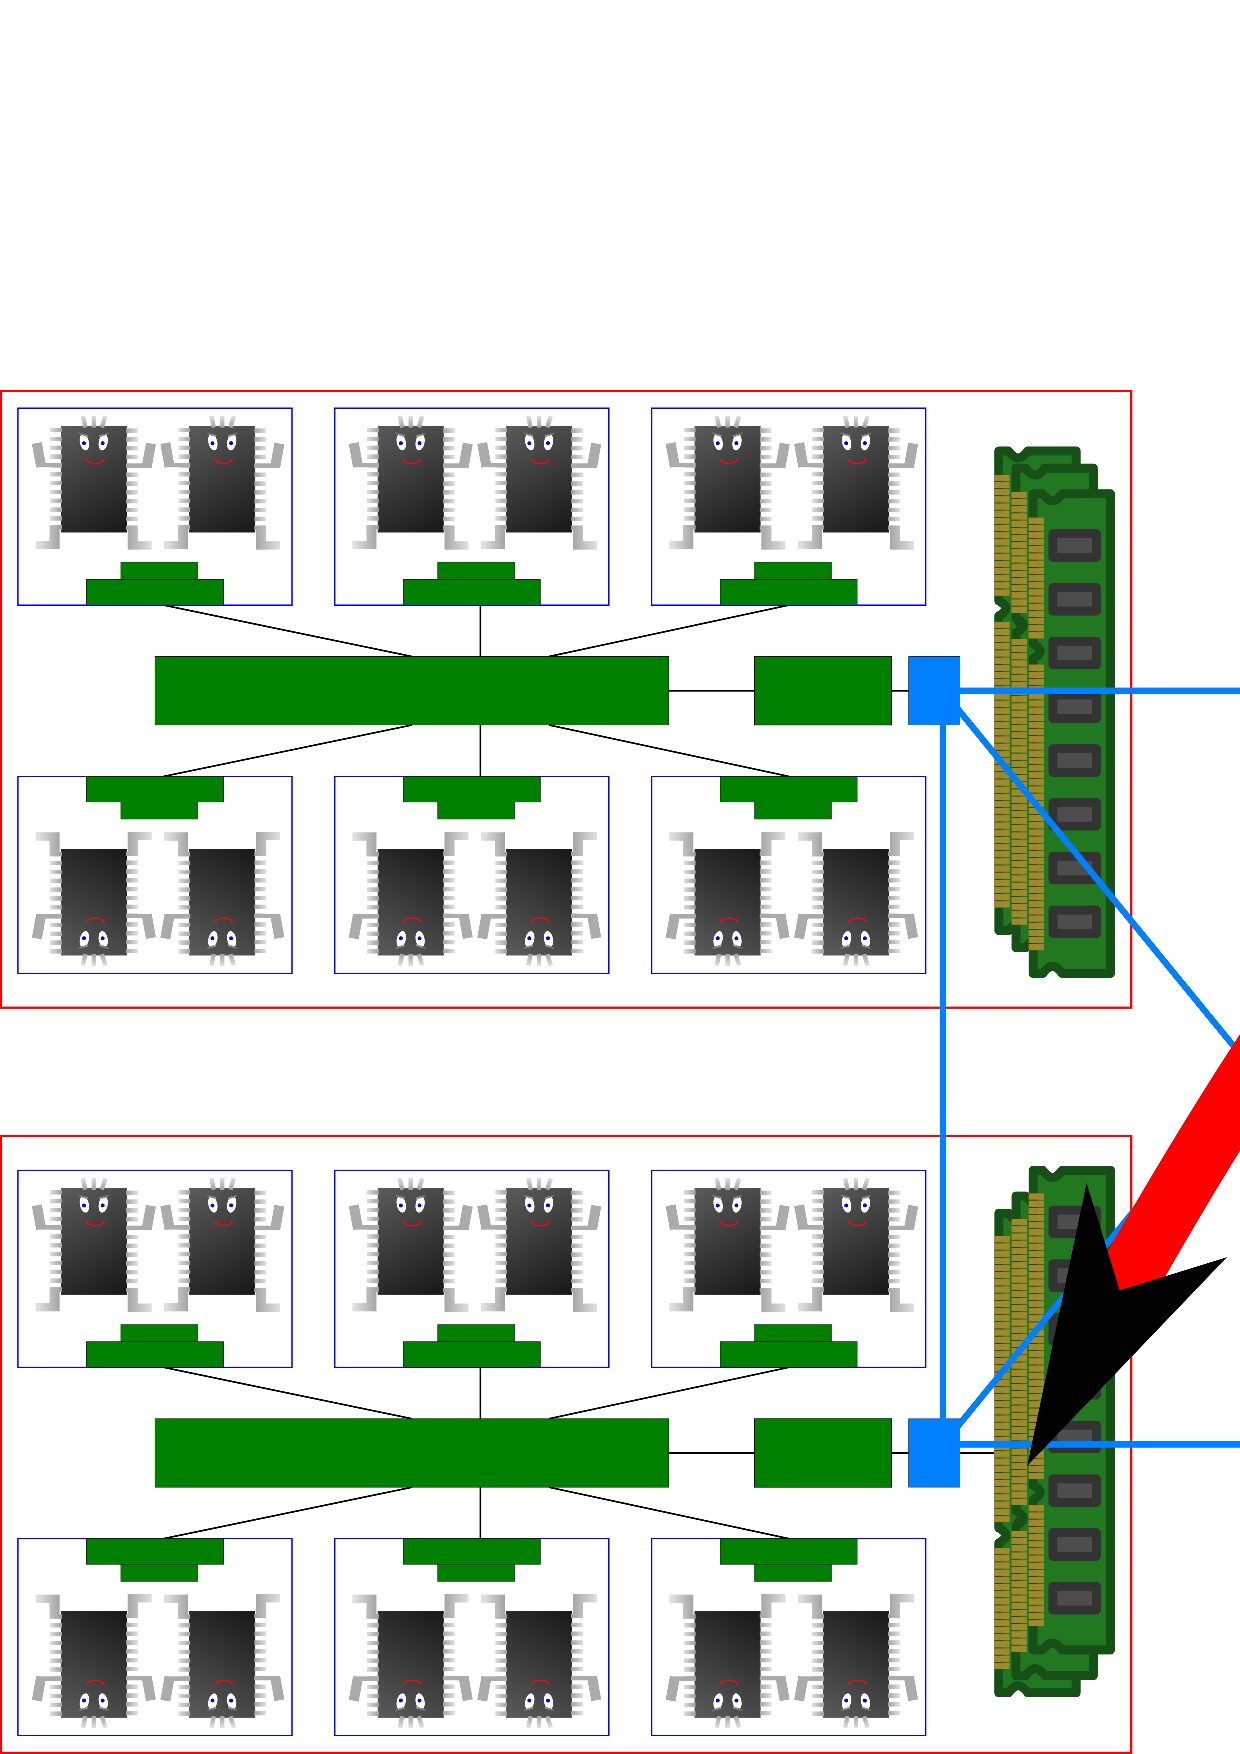
\includegraphics[width=\textwidth]{out/pdf/svg/diagram_multisocket_remote.pdf}
\end{column}
\end{columns}
\end{itemize}
\end{frame}

%=================================
\subsection{Bandwidth}
%=================================

%%%%%%%%%%%%%%%%%%%%%%%%%%%%%%%%%% 
\begin{frame}
\frametitle{Bandwidth of a random link list traversal}
\[ \mbox{bandwidth} = \frac{\mbox{total bytes read}}{\mbox{elapsed time}} \]
\begin{itemize}
\item in this experiment, we set record size $= 64$
\begin{columns}
\begin{column}{0.75\textwidth}
  %{\scriptsize\input{out/tex/data/mem/bw_local_remote_0.tex}}
  {\scriptsize\input{out/tex/data/08mem/bw_local_remote_big_0_1073741824.tex}}
  %out/tex/data/08mem/bw\_local\_remote\_big\_0\_1073741824.tex
  
\end{column}
\begin{column}{0.25\textwidth}
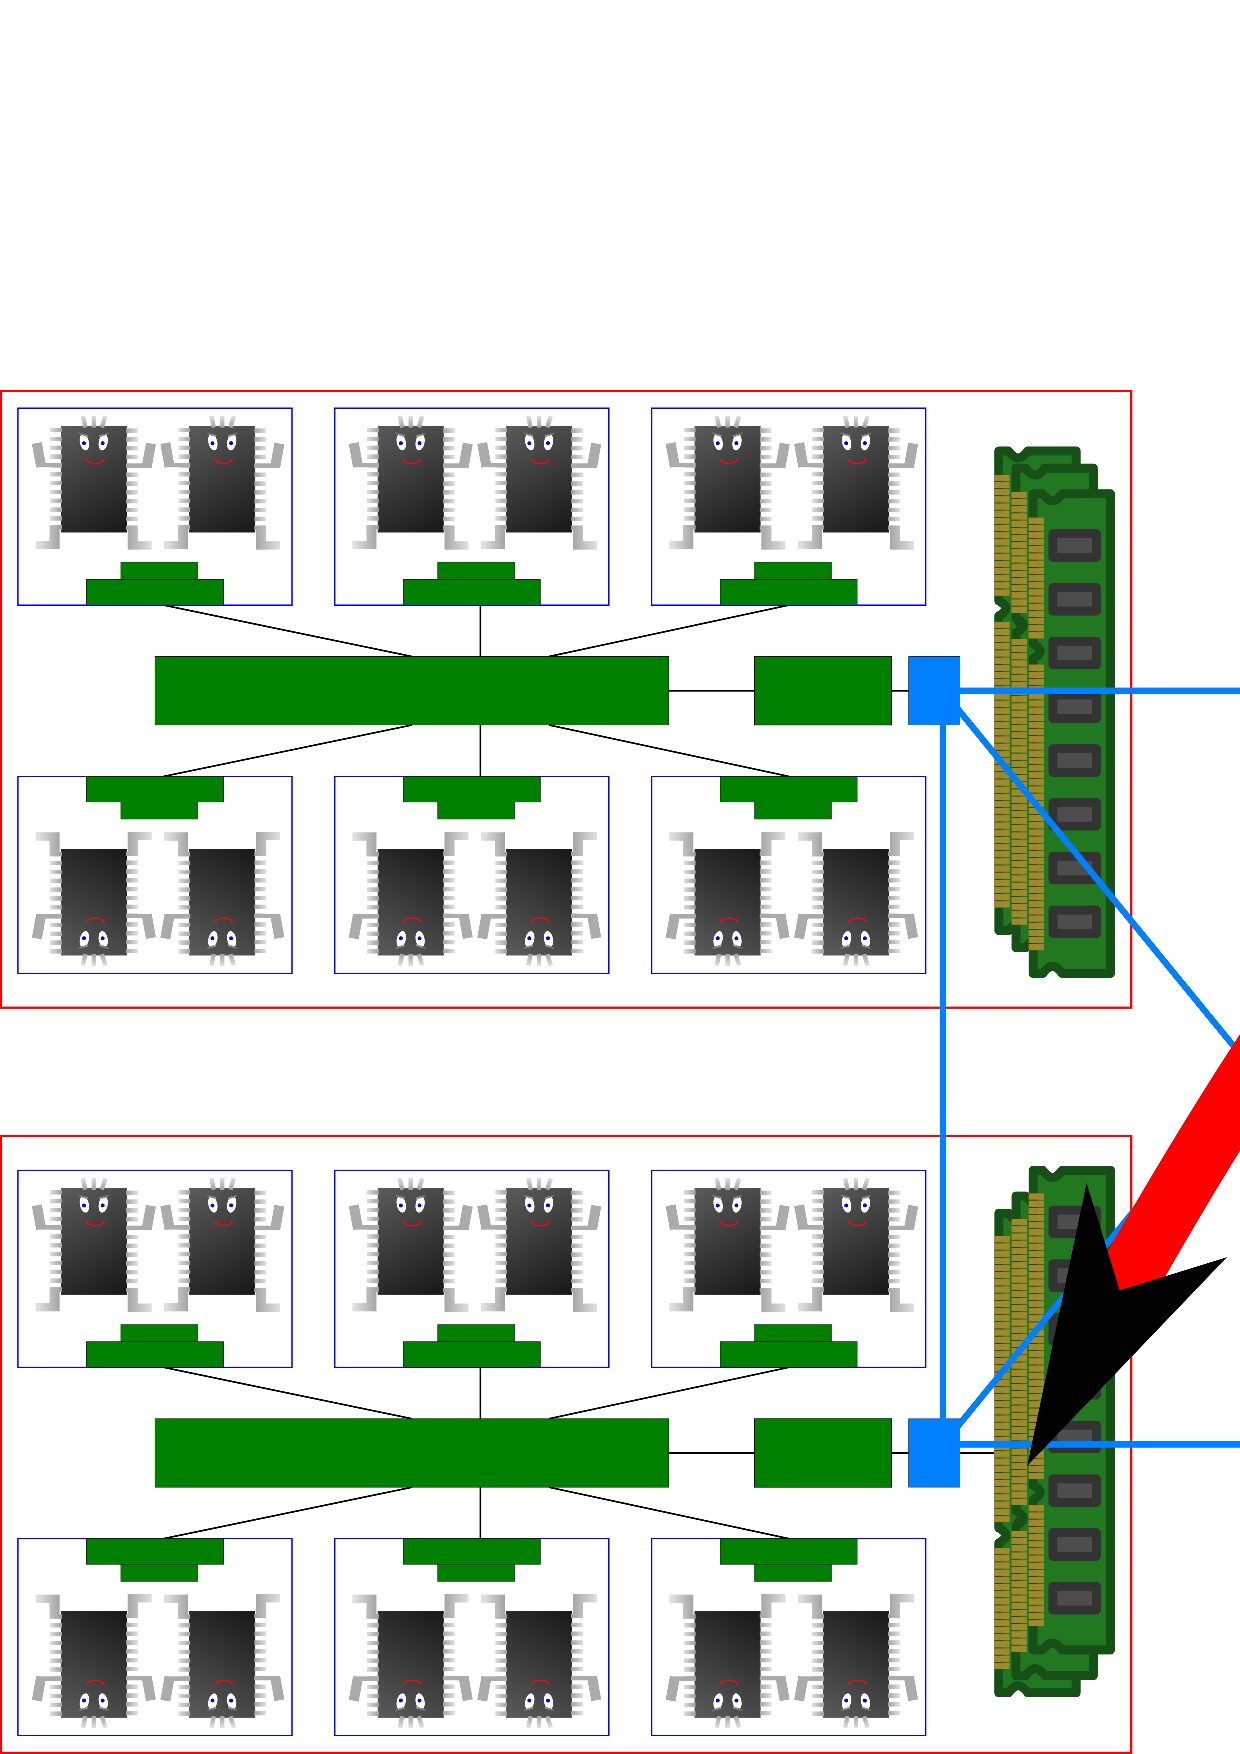
\includegraphics[width=\textwidth]{out/pdf/svg/diagram_multisocket_remote.pdf}
\end{column}
\end{columns}
\end{itemize}
\end{frame}

%%%%%%%%%%%%%%%%%%%%%%%%%%%%%%%%%% 
\begin{frame}
\frametitle{The ``main memory'' bandwidth}
\begin{itemize}
\item []
  % {\scriptsize\input{out/tex/data/mem/bw_local_remote_100000000.tex}}
  {\scriptsize\input{out/tex/data/08mem/bw_local_remote_big_33554432_1073741824.tex}}
  %out/tex/data/08mem/bw\_local\_remote\_big\_33554432\_1073741824.tex
\item $\ll$ the \texttt{memcpy} bandwidth we have seen ($\approx 4.5$ GB/s)
\item not to mention the ``memory bandwidth'' in the spec
\end{itemize}
\end{frame}

%%%%%%%%%%%%%%%%%%%%%%%%%%%%%%%%%% 
\begin{frame}[fragile]
\frametitle{Why is the bandwidth so low?}
\begin{itemize}
\item while traversing a single link list, 
  only a single record access (64 bytes) is ``in flight'' at a time

\begin{columns}
\begin{column}{0.5\textwidth}
\def\svgwidth{0.8\textwidth}
{\scriptsize \input{out/tex/svg/measure_latency.pdf_tex}}
\end{column}
\begin{column}{0.5\textwidth}
\includegraphics[width=0.8\textwidth]{out/pdf/svg/latency_very_large_1.pdf}
\end{column}
\end{columns}

\item in this condition,
\[ \mbox{bandwidth} = \frac{\mbox{a record size}}{\mbox{latency}} \]

\item e.g., take 115.45 ns as a latency
\[ \frac{64\mbox{ bytes}}{115.45\mbox{ ns}}
  \approx 0.55 \mbox{ GB/s} \]
\end{itemize}
\end{frame}

%%%%%%%%%%%%%%%%%%%%%%%%%%%%%%%%%% 
\begin{frame}[fragile]
\frametitle{How to get more bandwidth?}
\begin{itemize}
\item<1-> 
  just like flops/clock, the only way to get a better throughput (bandwidth) 
  is to perform \ao{\emph{many load operations concurrently}}

\begin{center}
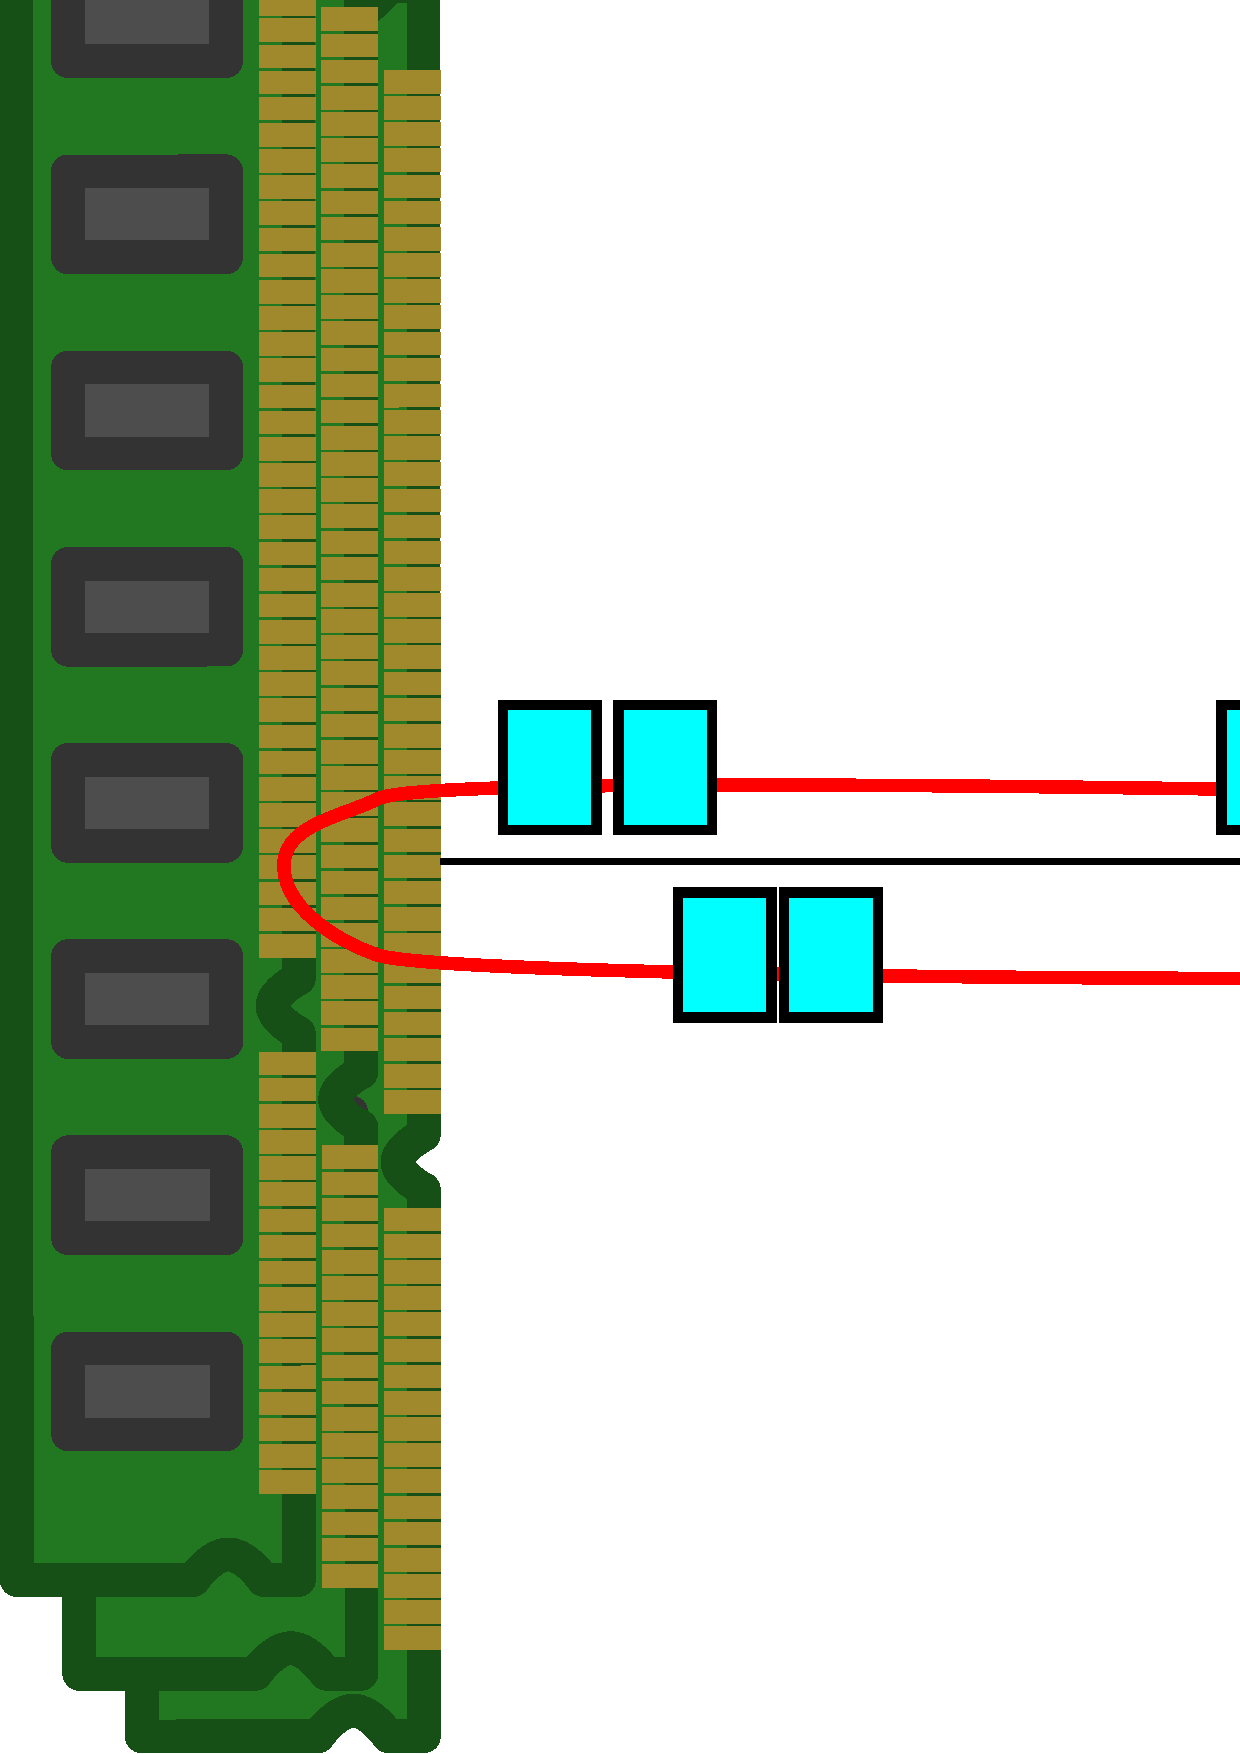
\includegraphics[width=0.35\textwidth]{out/pdf/svg/latency_very_large_2.pdf}
\end{center}

\item<2-> there are several ways to make it happen; 
  let's look at conceptually the most straightforward: traverse multiple lists
\begin{lstlisting}
for (@$N$@ times) {
  p1 = p1->next;
  p2 = p2->next;
     ...
}
\end{lstlisting}
\end{itemize}
\end{frame}

%=================================
\subsection{More bandwidth $=$ concurrent accesses}
%=================================

%%%%%%%%%%%%%%%%%%%%%%%%%%%%%%%%%% 
\begin{frame}[fragile]
\frametitle{The number of lists vs. bandwidth}
\begin{center}
  %{\scriptsize\input{out/tex/data/mem/bw_chains_local_0.tex}}
  {\scriptsize\input{out/tex/data/08mem/bw_chains_local_big_0_1073741824.tex}}
  %out/tex/data/08mem/bw\_chains\_local\_big\_0\_1073741824.tex
\end{center}
\begin{itemize}

\item let's zoom into ``main memory'' regime (size $>$ 100MB)
\end{itemize}
\end{frame}


%%%%%%%%%%%%%%%%%%%%%%%%%%%%%%%%%% 
\begin{frame}[fragile]
\frametitle{Bandwidth to the local main memory (not cache)}
\begin{itemize}
\item an almost proportional improvement up to $\sim$ 10 lists
\end{itemize}
\begin{center}
% {\scriptsize\input{out/tex/data/mem/bw_chains_local_100000000.tex}}
{\scriptsize\input{out/tex/data/08mem/bw_chains_local_big_33554432_1073741824.tex}}
% out/tex/data/08mem/bw\_chains\_local\_big\_33554432\_1073741824.tex
% {\scriptsize\input{out/tex/data/08mem/bw_chains_local_big_3_10.tex}}
\end{center}
\end{frame}

%%%%%%%%%%%%%%%%%%%%%%%%%%%%%%%%%% 
\begin{frame}[fragile]
\frametitle{Bandwidth to a remote main memory (not cache)}
\begin{itemize}
\item pattern is the same (improve up to $\sim$ 10 lists)
\item remember the remote latency is longer, so the bandwidth is
  accordingly lower
\end{itemize}
\begin{center}
  % {\scriptsize\input{out/tex/data/mem/bw_chains_remote_100000000.tex}}
  {\scriptsize\input{out/tex/data/08mem/bw_chains_remote_big_33554432_1073741824.tex}}
  %out/tex/data/08mem/bw\_chains\_remote\_big\_33554432\_1073741824.tex
\end{center}
\end{frame}

%%%%%%%%%%%%%%%%%%%%%%%%%%%%%%%%%% 
\begin{frame}
\frametitle{The number of lists vs. bandwidth}
\begin{itemize}
\item<1-> \ao{observation:} 
  bandwidth increase fairly proportionally to the number of lists,
  matching our understanding, \ldots
\begin{center}
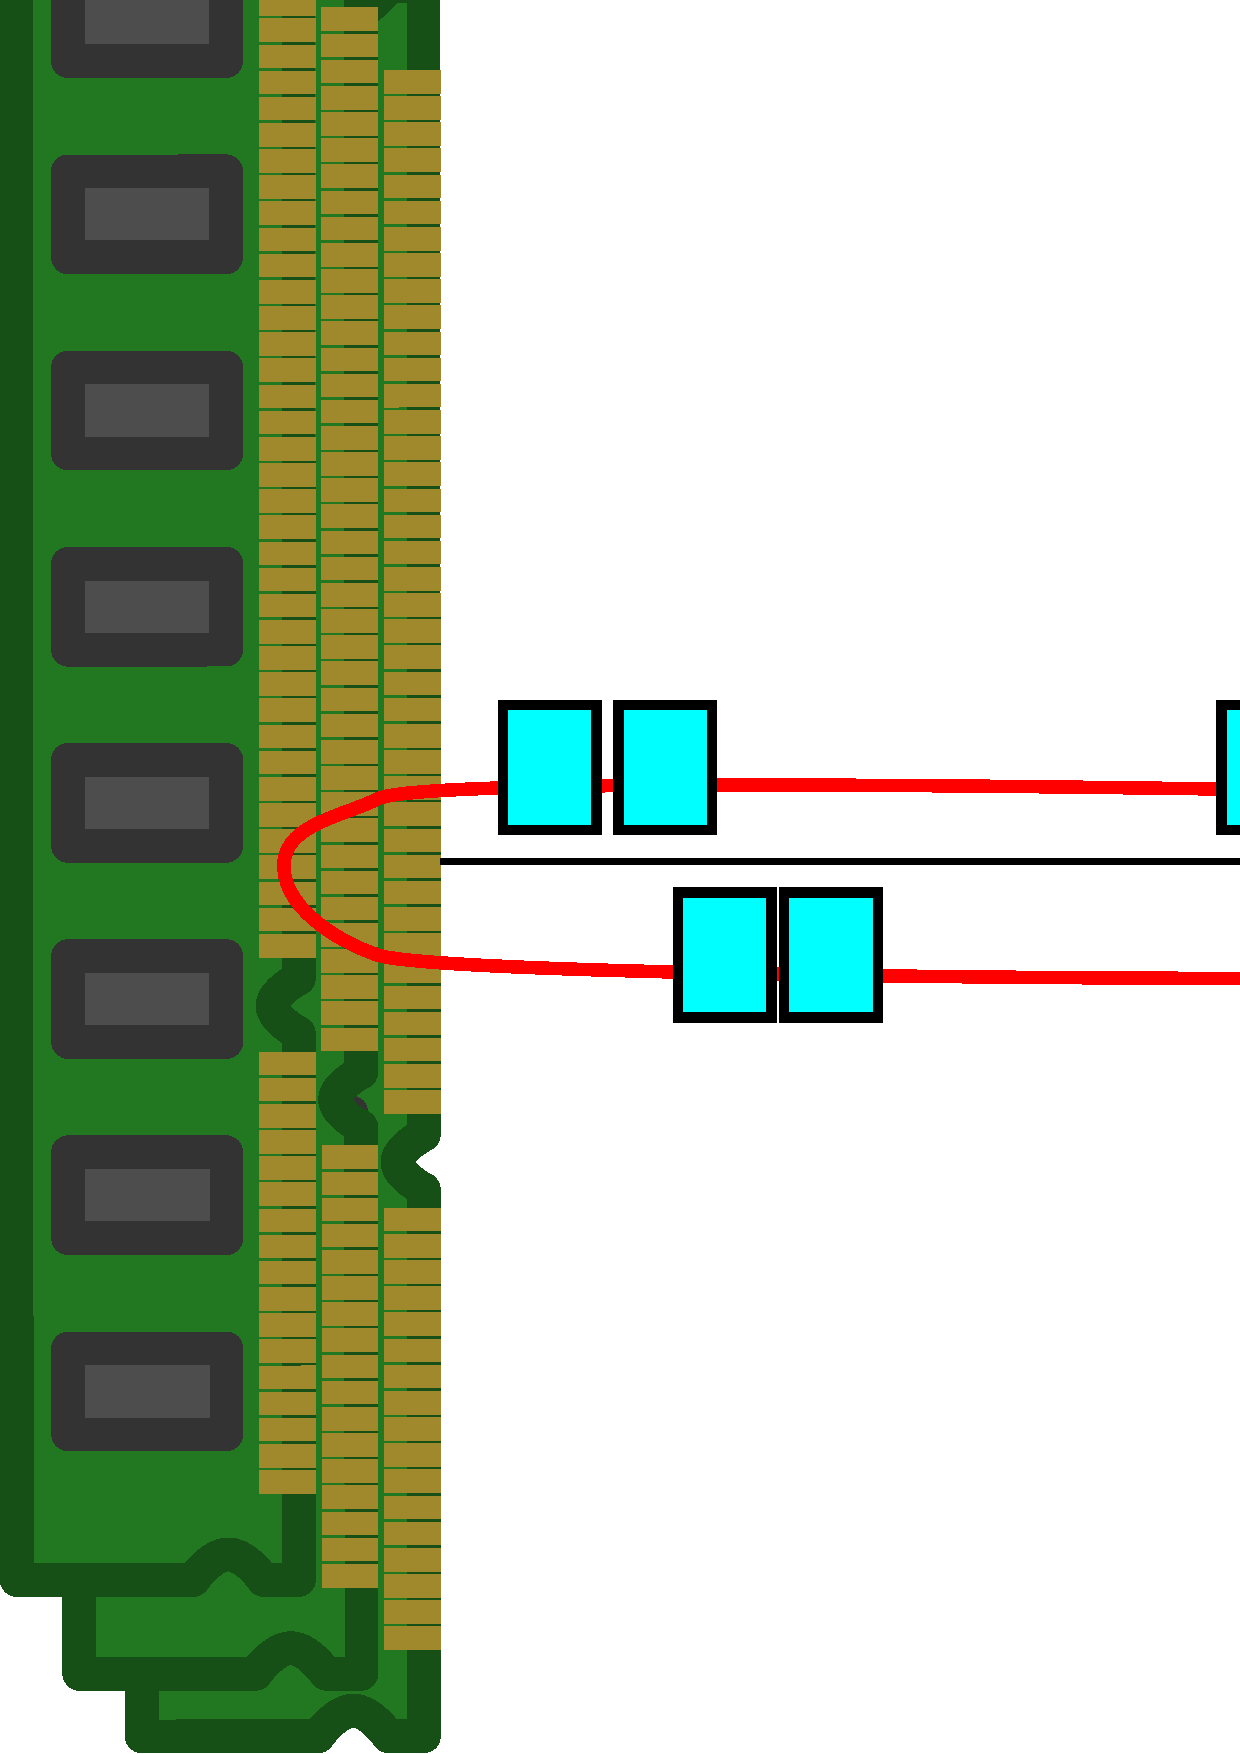
\includegraphics[width=0.4\textwidth]{out/pdf/svg/latency_very_large_2.pdf}
\end{center}
\item<2-> \ao{question:} \ldots but up to $\sim$ 10, why?
\item<3-> \ao{answer:} there is a limit in the number of 
  load operations in flight at a time
\end{itemize}
\end{frame}

%%%%%%%%%%%%%%%%%%%%%%%%%%%%%%%%%% 
\begin{frame}
\frametitle{Line Fill Buffer}
\begin{itemize}
\item<1-> \ao{\emph{Line fill buffer (LFB)}} is the processor resource that keeps track of outstanding cache misses, and its size is 10 in Haswell
  \begin{itemize}
  \item I could not find the definitive number for Skylake-X,
    but it will probably be the same
  \end{itemize}
\item<2-> this gives \ao{\em the maximum attainable bandwidth per core}
\[ \frac{\mbox{cache line size} \times \mbox{LFB size}}{\mbox{latency}} \]
\item<3-> this is what we've seen 
  (still much lower than what we see in the ``memory bandwidth'' in the spec sheet)
\item<4-> how can we go beyond this? $\Rightarrow$ 
  the only way is to \ao{\em use multiple cores} (covered later)
\end{itemize}
\end{frame}

%=================================
\section{Other ways to get more bandwidth}
%=================================

%%%%%%%%%%%%%%%%%%%%%%%%%%%%%%%%%% 
\begin{frame}[fragile]
\frametitle{Other ways to get more bandwidth}
\begin{itemize}
\item<1-> we've learned:
  \begin{itemize}
  \item maximum bandwidth $\approx$ 
    as many memory accesses as possible always in flight
  \item there is a limit due to LFB entries (10 in Haswell) 
  \end{itemize}

\item<2-> so far, we have achieved larger bandwidth by traversing
  multiple lists explicitly (sometimes difficult if not impossible to apply)

\item<3-> fortunately, the life is not always that
  tough; there are other ways to issue many memory accesses concurrently
  \begin{enumerate}
  \item make addresses sequential
  \item make address generations independent
  \item prefetch by software (make address generations go ahead)
  \item use multiple threads/cores
  \end{enumerate}
  
\item<4-> remember, all boil down to keep as many 
  memory accesses as possible (up to LFB entries) in flight 
\end{itemize}
\end{frame}

%=================================
\subsection{Make addresses sequential}
%=================================

%%%%%%%%%%%%%%%%%%%%%%%%%%%%%%%%%% 
\begin{frame}[fragile]
\frametitle{Make addresses sequential}
\begin{itemize}
\item again build a (single) linked list, but this time, {\tt p->next}
  always points to the immediately following block 

\item note that \aka{\em the instruction sequence
    is identical} to before; only addresses differ

\begin{center}
\def\svgwidth{0.5\textwidth}
{\footnotesize \input{out/tex/svg/measure_latency_prefetch.pdf_tex}}
\end{center}
\begin{center}
  vs.
\end{center}
\begin{center}
\def\svgwidth{0.5\textwidth}
{\scriptsize \input{out/tex/svg/measure_latency.pdf_tex}}
\end{center}
\end{itemize}
\end{frame}


%%%%%%%%%%%%%%%%%%%%%%%%%%%%%%%%%% 
\begin{frame}
\frametitle{Bandwidth of traversing address-ordered list}

\begin{itemize}
\item a factor of 10 faster than random case, but this time
  with only a single list
\begin{center}
  %{\scriptsize\input{out/tex/data/mem/sorted_0.tex}}
  {\scriptsize\input{out/tex/data/08mem/sorted_big_0_1073741824.tex}}
  %out/tex/data/08mem/sorted\_big\_0\_1073741824.tex
\end{center}

\end{itemize}
\end{frame}

%%%%%%%%%%%%%%%%%%%%%%%%%%%%%%%%%% 
\begin{frame}
\frametitle{The reason this is faster}
\begin{itemize}
\item \ao{\em hardware prefetcher}
\item CPU watches the sequence of addresses accessed
\item sequential addresses (addresses of a small constant stride) 
  trigger CPU's hardware prefetcher
\item CPU issues load instruction ahead of actual data stream
  on your behalf, to keep the maximum number of loads in flight
\end{itemize}

\begin{center}
\def\svgwidth{0.5\textwidth}
{\footnotesize \input{out/tex/svg/measure_latency_prefetch.pdf_tex}}
\end{center}

\end{frame}

%=================================
\subsection{Make address generations independent}
%=================================

%%%%%%%%%%%%%%%%%%%%%%%%%%%%%%%%%% 
\begin{frame}[fragile]
\frametitle{Make address generations independent}
\begin{itemize}

\item if addresses of memory accesses can be
  computed without values returned from
  previous loads, CPU can issue them concurrently

\begin{lstlisting}
for (@$N$@ times) {
  j = ... /* not use a[@$\cdot$@] */
  a[j];
}
\end{lstlisting}

\begin{center}
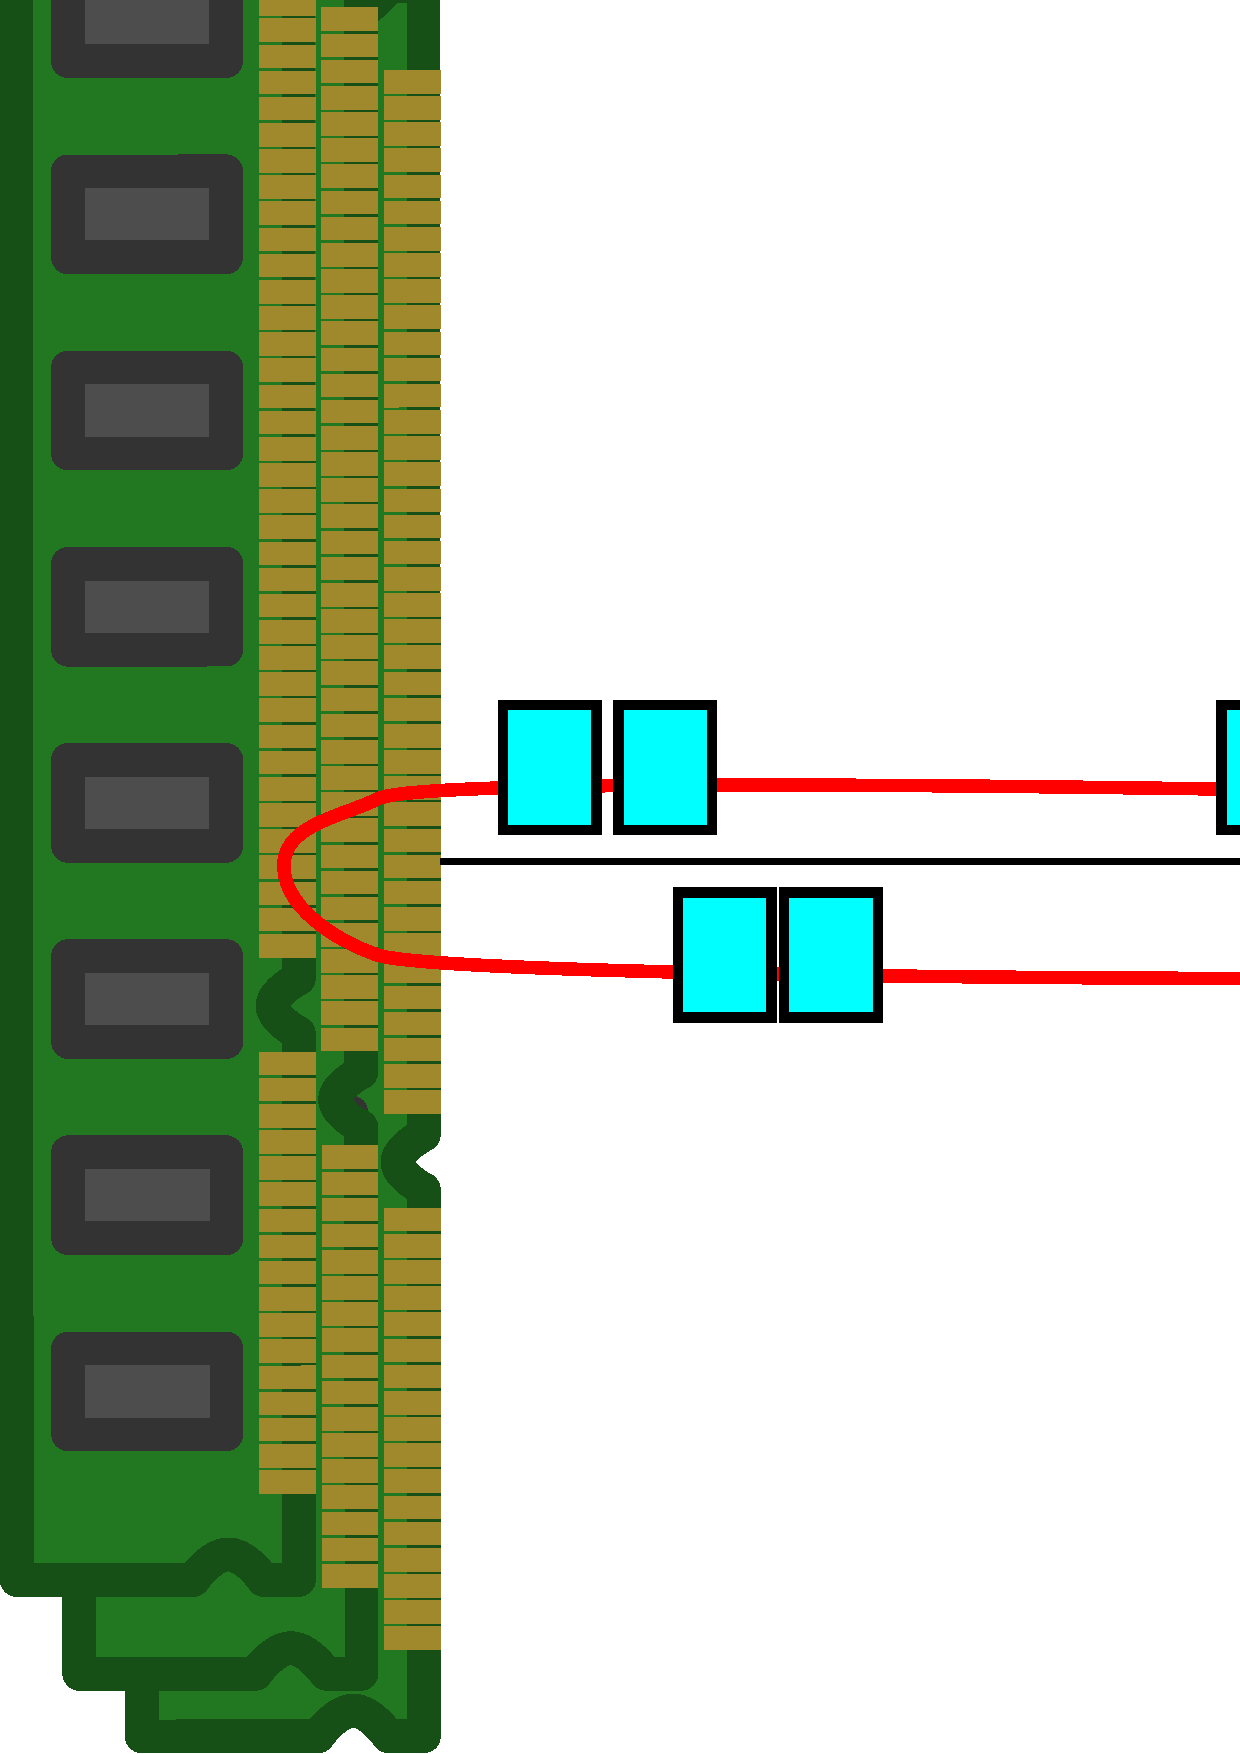
\includegraphics[width=0.4\textwidth]{out/pdf/svg/latency_very_large_2.pdf}
\end{center}

\item note: it's \ao{\emph{not}} a prefetch (but a real fetch)
\end{itemize}
\end{frame}


%%%%%%%%%%%%%%%%%%%%%%%%%%%%%%%%%% 
\begin{frame}[fragile]
\frametitle{Bandwidth when not traversing a list}
\begin{itemize}
\item ptrchase : chase pointers of a random list
\item random : access random addresses, but w/o pointer chasing
\item sequential : access sequential addresses, w/o pointer chasing
\end{itemize}
\begin{center}
  %{\scriptsize\input{out/tex/data/mem/methods_0.tex}}
  {\scriptsize\input{out/tex/data/08mem/methods_big_0_1073741824.tex}}
  %out/tex/data/08mem/methods\_big\_0\_1073741824.tex
\end{center}
\end{frame}

%%%%%%%%%%%%%%%%%%%%%%%%%%%%%%%%%% 
\begin{frame}[fragile]
\frametitle{Main memory bandwidth}
\begin{itemize}
\item pointer chase $\ll$ random $<$ sequential
\item random is $\approx$ 5x faster than traversing a single random list
\begin{center}
  % {\scriptsize\input{out/tex/data/mem/methods_100000000.tex}}
  {\scriptsize\input{out/tex/data/08mem/methods_big_33554432_1073741824.tex}}
  %out/tex/data/08mem/methods\_big\_33554432\_1073741824.tex
\end{center}
\end{itemize}
\end{frame}

%%%%%%%%%%%%%%%%%%%%%%%%%%%%%%%%%% 
\begin{frame}
\frametitle{Main memory bandwidth (random vs. sequential)}
\begin{itemize}
\item sequential gets $\approx$ 3x more bandwidth than random
\item may not be as bad as you thought?
\item but why is there \ao{\emph{any}} difference, 
  if both have the same number of loads in flight?
\end{itemize}
\begin{center}
  % {\scriptsize\input{out/tex/data/mem/methods_100000000.tex}}
  {\scriptsize\input{out/tex/data/08mem/methods_big_33554432_1073741824.tex}}
  %out/tex/data/08mem/methods\_big\_33554432\_1073741824.tex
\end{center}
\end{frame}

%%%%%%%%%%%%%%%%%%%%%%%%%%%%%%%%%% 
\begin{frame}
\frametitle{Random (index) vs. sequential}
\begin{itemize}
\item if both can have up to 10 (LFB entries)
  outstanding L1 cache misses, why is there \ao{\it any} diffference?
  
\item I don't have a definitive answer, but presumably,
  \begin{itemize}
  \item the hardware prefetcher happens at multiple levels
    ($\rightarrow$ L1 and $\rightarrow$ L2)
  \item prefetchers to L2 are not subject of the LFP entries limit
    (the limit will be slightly more)
  \item prefething to L2 make effective latency to the processor smaller
  \end{itemize}
\end{itemize}
\end{frame}

%%%%%%%%%%%%%%%%%%%%%%%%%%%%%%%%%% 
\begin{frame}
\frametitle{When ``random access'' is really bad}
\begin{itemize}
\item in practice, when random vs. sequential makes a large ($\gg$ 2) 
difference, it's because 
\[ \mbox{a single element} < \mbox{a single cache line} \]

\item recall that touching a single byte in a cache line still 
  brings the whole line (64 bytes)

\item e.g., if you access an array of \texttt{float} (4 bytes) randomly,
  the bandwidth of \ao{\emph{useful}} data 
  is amplified by a factor of 16 ($= 64/4$)
\end{itemize}
\end{frame}

%=================================
\subsection{Prefetch by software (make address generations go ahead)}
%=================================

%%%%%%%%%%%%%%%%%%%%%%%%%%%%%%%%%% 
\begin{frame}[fragile]
\frametitle{Software prefetch}
\begin{itemize}
\item<1-> hardware prefetch happens only for sequential 
  (a small constant stride) accesses
\item<1-> for other patterns, you the programmer 
  may know addresses you are going to access soon
\item<2-> \ao{\emph{if}} you can generate those addresses 
  much ahead of actual load instructions, you can \ao{\emph{prefetch}} them
\item<3-> instructions:
  \begin{itemize}
  \item prefetcht\{0,1,2\}
  \item prefetchnta
  \end{itemize}
\item<4-> intrinsics:
\begin{lstlisting}
__builtin_prefetch(@$a$@ @[@, @{\it rw}@, @{\it hint}@ @]@)
\end{lstlisting}
\end{itemize}
\end{frame}


%%%%%%%%%%%%%%%%%%%%%%%%%%%%%%%%%% 
\begin{frame}[fragile]
\frametitle{How to apply software prefetch?}
\begin{itemize}
\item<1-> truth is, there are actually not many cicumstances this is useful
\item<2-> why?
  by the time you can \ao{\emph{prefetch}} it, 
  you can likewise \ao{\emph{load}} it!
\item<3-> in our example, 
  \begin{itemize}
  \item<3-> no point in applying it to index-based accesses 
    (CPU will issue many load instructions already)
  \item<4-> on the other hand, it's difficult to apply it to list traversal
    (it takes equally long time to generate address to prefetch)
  \end{itemize}
\item<5-> the only way to apply it is to change the data structure of the linked list
\item<6-> but how?
\end{itemize}
\end{frame}


%%%%%%%%%%%%%%%%%%%%%%%%%%%%%%%%%% 
\begin{frame}[fragile]
\frametitle{How to apply software prefetch?}
\begin{itemize}
\item have another pointer pointing many elements ahead
\begin{lstlisting}
for (@$N$@ times) {
  p = p->next;
  prefetch(p->prefetch);
}
\end{lstlisting}

\item it should point to 
  $Q$ elements ahead to have $Q$ concurrent accesses in flight
\end{itemize}

\begin{center}
\def\svgwidth{\textwidth}
{\scriptsize\input{out/tex/svg/sw_prefetch.pdf_tex}}
\end{center}
\end{frame}

%%%%%%%%%%%%%%%%%%%%%%%%%%%%%%%%%% 
\begin{frame}[fragile]
\frametitle{Result}

\begin{center}
  %{\scriptsize\input{out/tex/data/mem/bw_prefetch_100000000.tex}}
  {\scriptsize\input{out/tex/data/08mem/bw_prefetch_big_33554432_1073741824.tex}}
  %out/tex/data/08mem/bw\_prefetch\_big\_33554432\_1073741824.tex
\end{center}
\end{frame}

%%%%%%%%%%%%%%%%%%%%%%%%%%%%%%%%%% 
\begin{frame}
\frametitle{Summary: bandwidth of various access patterns}

\begin{itemize}
\item sequential (w/o pointer chase) $>$ sorted list
\item [] $>$ random (w/o pointer chase) 
$\approx$ 5 random lists $\approx$ a random list $+$ software prefetch
\item [] $>$ a random list
\end{itemize}

\begin{center}
  %{\scriptsize\input{out/tex/data/mem/summary_100000000.tex}}
  {\scriptsize\input{out/tex/data/08mem/summary_big_33554432_1073741824.tex}}
  %out/tex/data/08mem/summary\_big\_33554432\_1073741824.tex
\end{center}
\end{frame}

%=================================
\subsection{Use multiple threads/cores}
%=================================

%%%%%%%%%%%%%%%%%%%%%%%%%%%%%%%%%% 
\begin{frame}
\frametitle{Memory bandwidth with multiple cores}
\begin{itemize}
\item the bandwidth to a single core is limited by LFB entries
  and is much lower than the memory bandwidth itself
  \[ \frac{\mbox{transfer (line) size }
      \times \mbox{ LFB entries}}{\mbox{latency}} \]
\item you can go beyond that by using multiple cores
  and \ao{\it this is the only way}
\end{itemize}
\end{frame}

%%%%%%%%%%%%%%%%%%%%%%%%%%%%%%%%%% 
\begin{frame}
\frametitle{Memory bandwidth with multiple cores}
\begin{itemize}
\item run up to 16 threads,
\item each running on a
  distinct physical core of a single socket
\item allocate all the data on the same socket ({\tt numactl -N 0 -i 0})
\item note: they are still random pointer chasing
\end{itemize}
\begin{center}
{\scriptsize\input{out/tex/data/08mem/bw_threads_big_33554432_1073741824.tex}}
%out/tex/data/08mem/bw\_threads\_big\_33554432\_1073741824.tex
\end{center}
\end{frame}

%%%%%%%%%%%%%%%%%%%%%%%%%%%%%%%%%% 
\begin{frame}
\frametitle{With random indexing and sequential accesses}
\begin{itemize}
\item similar experiments with random indexing/sequential accesses
\item $\sim$ 80 GB/sec with sequential accesses by $\geq$ 12 threads
\item the theoretical peak is
  \[ 8 \mbox{ bytes } \times 2.666 \mbox{ GHz }
    \times 6 \mbox{ channels } = 128 \mbox{ GB/sec} \]
  
\begin{center}
\def\svgwidth{0.7\textwidth}
{\scriptsize\input{out/tex/data/08mem/bw_methods_threads_big_33554432_1073741824.tex}}
%out/tex/data/08mem/bw\_methods\_threads\_big\_33554432\_1073741824.tex
\end{center}

\end{itemize}
\end{frame}


%%%%%%%%%%%%%%%%%%%%%%%%%%%%%%%%%% 
\begin{frame}
\frametitle{With multiple CPU sockets}
\begin{itemize}
\item the total bandwidth depends on how to place threads and data
\begin{tabular}{|c|c|c|c|c|} \hline
threads\textbackslash data & CPU $x$ & CPU $y$ & all CPUs & local CPU  \\\hline
CPU $x$             & 1-local & 1-remote  & 1-all   & 1-local \\
all CPUs            & all-1   & all-1     & all-all & all-local \\\hline
\end{tabular}

\item control threads/data placement by {\tt numactl} command
\item combine it with {\tt OMP\_PROC\_BIND=true} to get a desired effect
\end{itemize}

\begin{center}
%\def\svgwidth{0.4\textwidth}
\includegraphics[width=0.6\textwidth]{out/pdf/svg/diagram_multisocket.pdf}
\end{center}
\end{frame}

%%%%%%%%%%%%%%%%%%%%%%%%%%%%%%%%%% 
\begin{frame}[fragile]
\frametitle{{\tt numactl} command (1)}
\begin{itemize}
\item usage (see {\tt man numactl} for details)
\begin{lstlisting}
$ numactl @{\it options}@ command    
\end{lstlisting} %$
\begin{itemize}
\item for underlying system calls, see {\tt man -s 3 numa}
\end{itemize}

\item processors
  \begin{itemize}
\item {\tt -N} $x$ runs threads only on the CPU(s) $x$. e.g.,
\begin{lstlisting}
$ numactl @\ao{\tt -N 0}@ @{\it command}@   # threads on CPU 0
\end{lstlisting} %$
\item {\tt --physcpubind} $x$ runs threads only on {\it core(s)} $x$. e.g.,
\begin{lstlisting}
# threads on cores 0-11 and 16-27    
$ numactl @\ao{\tt --physcpubind 0-11,16-27}@ @{\it command}@
\end{lstlisting} %$
\end{itemize}
\end{itemize}
\end{frame}

%%%%%%%%%%%%%%%%%%%%%%%%%%%%%%%%%% 
\begin{frame}[fragile]
\frametitle{{\tt numactl} command (2)}
\begin{itemize}
\item memory (data)
  \begin{itemize}
  \item {\tt -i} $y$ allocates data (physical pages) on CPU(s) $y$
\begin{lstlisting}
$ numactl @\ao{\tt -i 0,1}@ @{\it command}@ # data on CPU 0 or 1
$ numactl @\ao{\tt -i all}@ @{\it command}@ # data on all CPUs
\end{lstlisting} %$ 
\item {\tt -l} allocates physical pages to the
  CPU that touches the page for the first time
  (\ao{\it first touch policy}; the default policy of Linux)
\begin{lstlisting}
$ numactl @\ao{\tt -l}@ @{\it command}@
\end{lstlisting} %$
\end{itemize}
\end{itemize}
\end{frame}

%%%%%%%%%%%%%%%%%%%%%%%%%%%%%%%%%% 
\begin{frame}
\frametitle{About the {\tt -l} option}
\begin{itemize}
\item {\tt -l} (equivalent: {\tt --localalloc})
  allocates the physical page for a logical page
  \ao{\it on the CPU that first touches it (first touch)}
  
\item allocated physical pages do not move thereafter
  (unless you do so by {\tt move\_pages()} system call)

\item don't be fooled by its name;
  it is \aka{\it not} a policy that automagically
  makes memory accesses local

\item quite contrary, it often makes a \aka{\it hotspot} in a single CPU,
  especially when only one thread initializes (first-touches) the data

\item {\tt -iall} is not optimal, but often much safer
  for parallel applications
\end{itemize}
\end{frame}

%%%%%%%%%%%%%%%%%%%%%%%%%%%%%%%%%% 
\begin{frame}[fragile]
\frametitle{OpenMP thread placement}
\begin{itemize}
\item combine them with {\tt OMP\_NUM\_THREADS=}
  and {\tt OMP\_PROC\_BIND=true}
  to get a desired effect. e.g.,
\begin{lstlisting}
$ OMP_NUM_THREADS=48 OMP_PROC_BIND=true numactl --physcpubind 0-11,16-27,32-43,48-59 -l @{\it command}@
\end{lstlisting} %$
\end{itemize}
to
\begin{itemize}
\item run 12 threads on each CPU (of a host in the big partition)
\item and use the first touch policy
\end{itemize}
\end{frame}

%%%%%%%%%%%%%%%%%%%%%%%%%%%%%%%%%% 
\begin{frame}
  \frametitle{Achieved bandwidth}
  \begin{itemize}
  \item Skylake X 6130 $\times 4$ CPUs (a host of the ``big'' partition)
  \item use 12 (of 16) cores on each CPU 
  \item in each measurement,
    each thread reads $\approx$ 640MB sequentially 10 times
  \end{itemize}

  \begin{center}
  \begin{tabular}{|l|r|r|}\hline
    setting   & threads & bandwidth (GB/sec) \\\hline
    1-local   & 12      & 85  \\
    1-remote  & 12      & \aka{16}  \\
    1-all     & 12      & 57  \\
    all-1     & 48      & \aka{2}   \\
    all-all   & 48      & 97  \\
    all-local & 48      & \ao{320} \\\hline
  \end{tabular}
  \end{center}
  
\end{frame}

%%%%%%%%%%%%%%%%%%%%%%%%%%%%%%%%%% 
\begin{frame}
  \frametitle{Remarks on remote access bandwidths}
  \begin{itemize}
  \item \aka{\it numbers for remote accesses} are ridiculously low
  \item the measurement is repeated 6 times and there were almost no
    variations in the result (within a few per cents)
  \item I am suspecting a wrong BIOS snoop setting
    (\url{https://software.intel.com/en-us/forums/software-tuning-performance-optimization-platform-monitoring/topic/602160})
  \end{itemize}

  \begin{center}
  \begin{tabular}{|l|r|r|}\hline
    setting   & threads & bandwidth (GB/sec) \\\hline
    1-local   & 12      & 85  \\
    1-remote  & 12      & \aka{16}  \\
    1-all     & 12      & 57  \\
    all-1     & 48      & \aka{2}   \\
    all-all   & 48      & 97  \\
    all-local & 48      & \ao{320} \\\hline
  \end{tabular}
  \end{center}
  
\end{frame}

%=================================
\section{How costly is it to communicate between threads?}
%=================================

%%%%%%%%%%%%%%%%%%%%%%%%%%%%%%%%%% 
\begin{frame}
\frametitle{Shared memory}
\begin{itemize}
\item if thread $P$ writes to an address $a$ 
  and then another thread $B$ reads from $a$,
  $Q$ observes the value written by $P$

\begin{center}
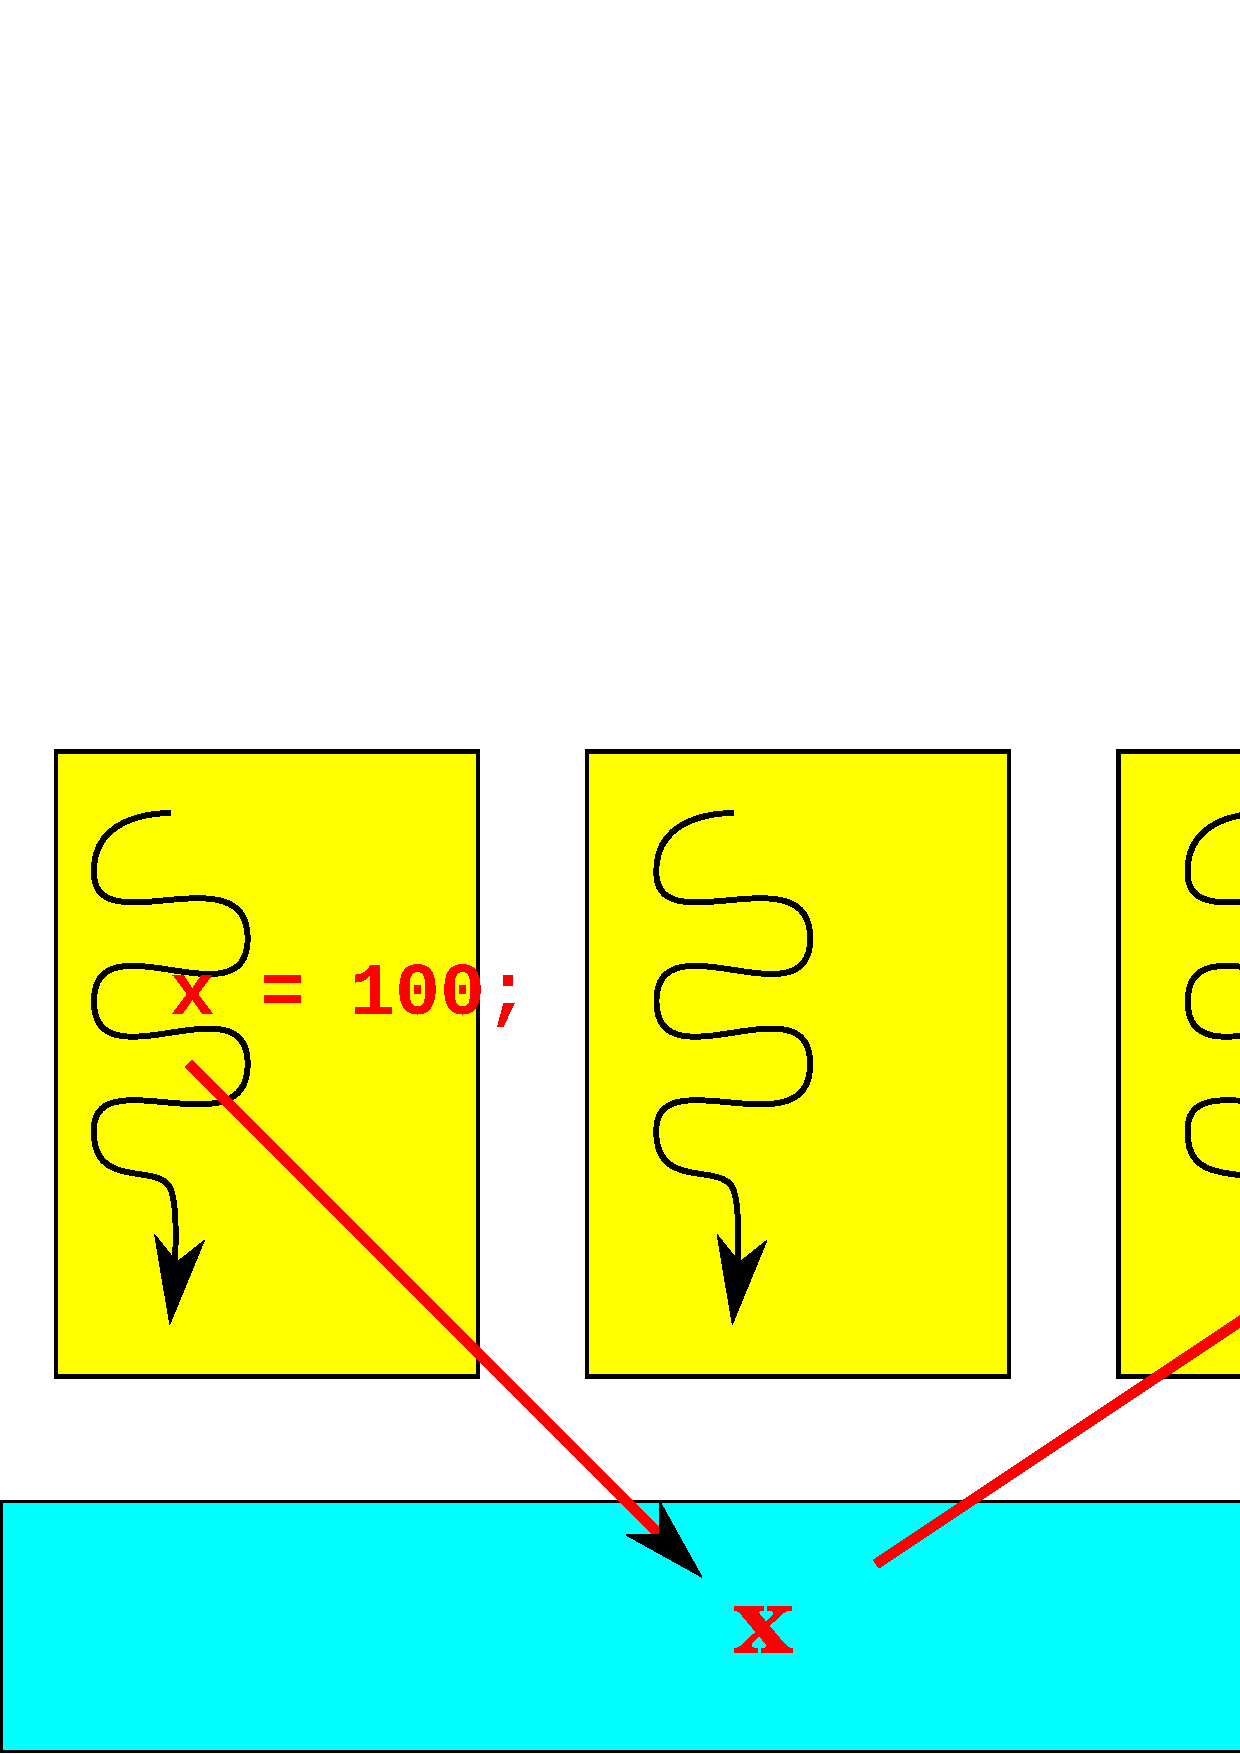
\includegraphics[width=0.3\textwidth]{out/pdf/svg/shmem_programming_easy.pdf}
\end{center}

\item<2-> ordinary load/store instructions accomplish this
  \ao{\em (hardware shared memory)}

\item<2-> this should not be taken for granted;
  processors have {\em caches} and a
  single address may be cached by multiple
  cores/sockets

\end{itemize}
\end{frame}

%%%%%%%%%%%%%%%%%%%%%%%%%%%%%%%%%% 
\begin{frame}
\frametitle{Shared memory}
\begin{itemize}
\item $\Rightarrow$ processors sharing memory are
  running a complex, \ao{\em cache coherence
    protocol} to accomplish this

\item roughly, 
  \begin{enumerate}
  \item<2-> a write to an address by a
    processor ``invalidates'' all other cache lines
    holding the address, so that no caches hold
    ``stale'' values
  \item<3-> a read to an invalid line causes a miss and 
    searches for a cache holding its ``valid'' value
  \end{enumerate}
\end{itemize}

\begin{center}
\only<1>{\includegraphics[width=0.4\textwidth]{out/pdf/svg/diagram_multisocket.pdf}}%
\only<2>{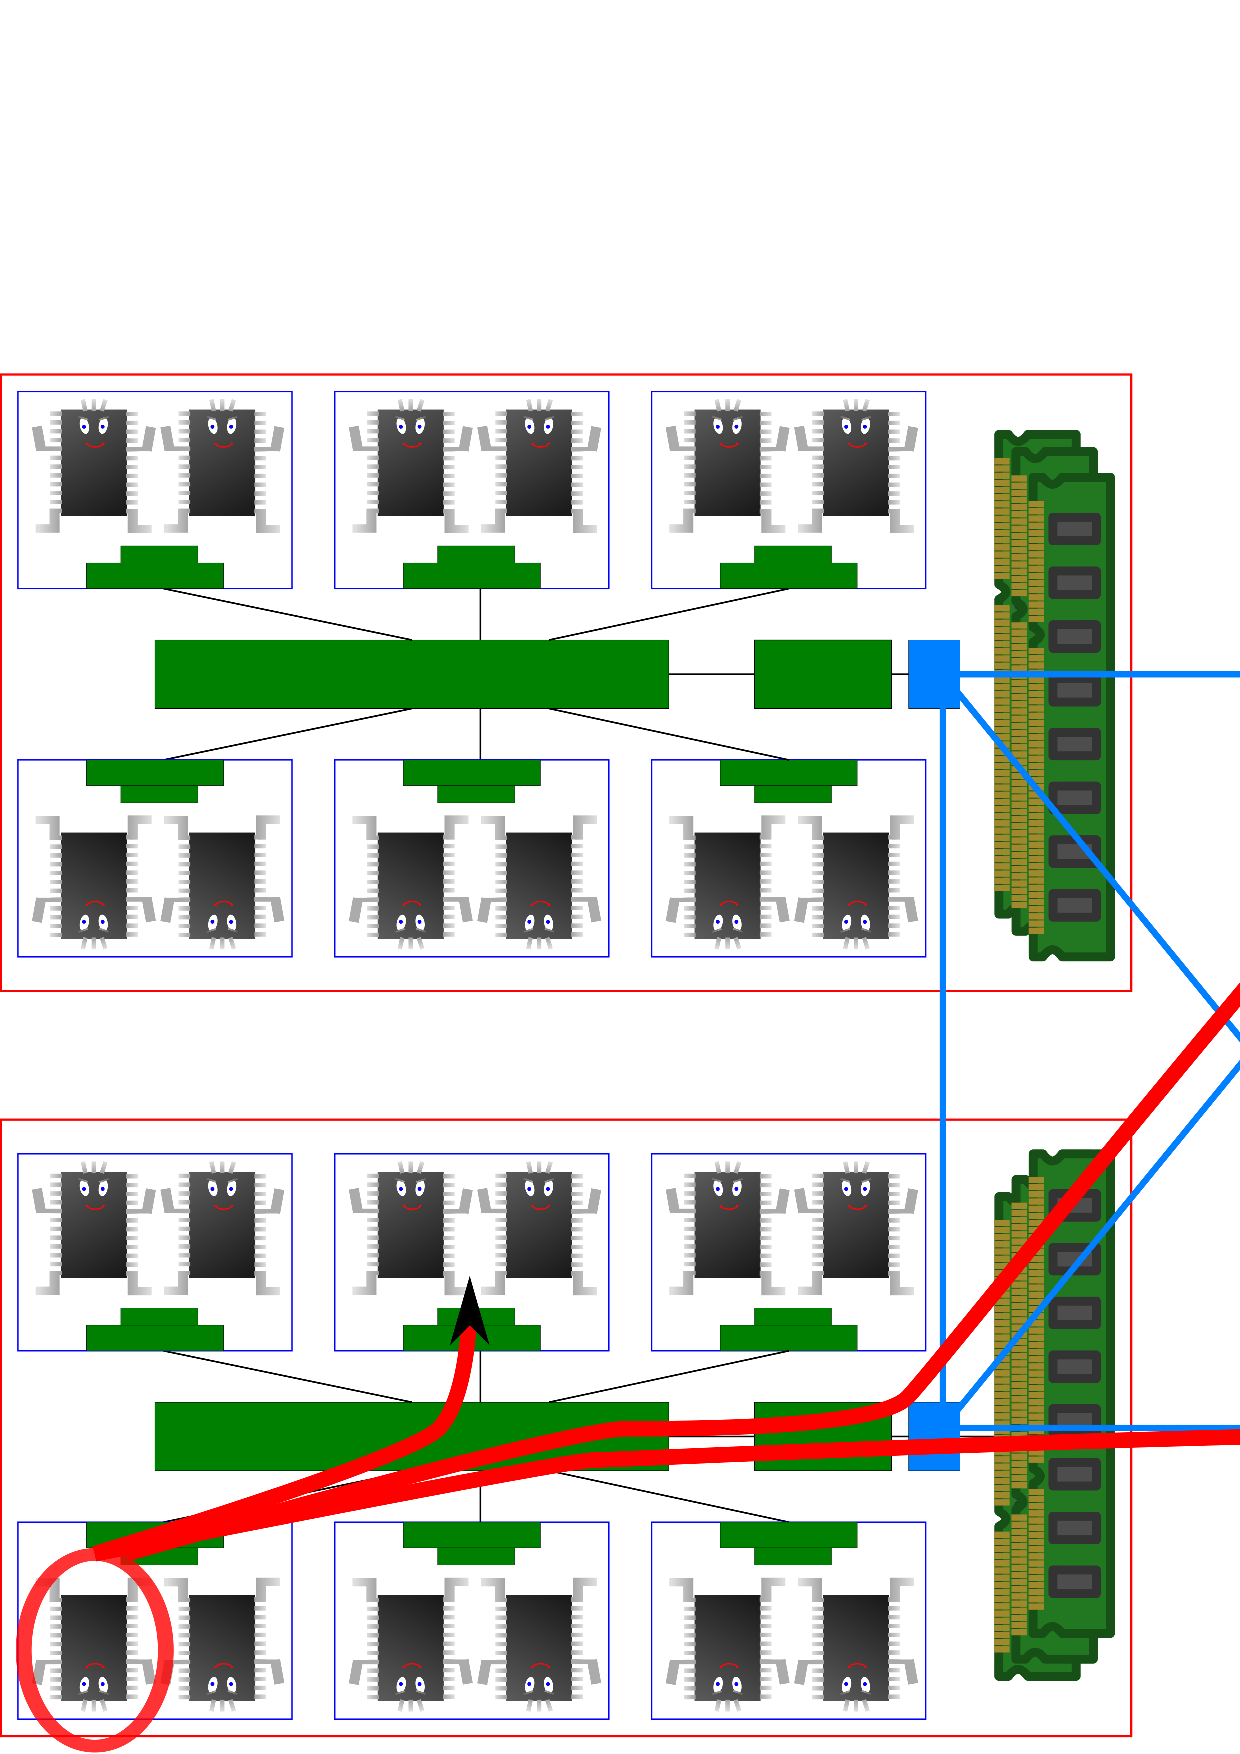
\includegraphics[width=0.4\textwidth]{out/pdf/svg/cache_coherent_write.pdf}}%
\only<3>{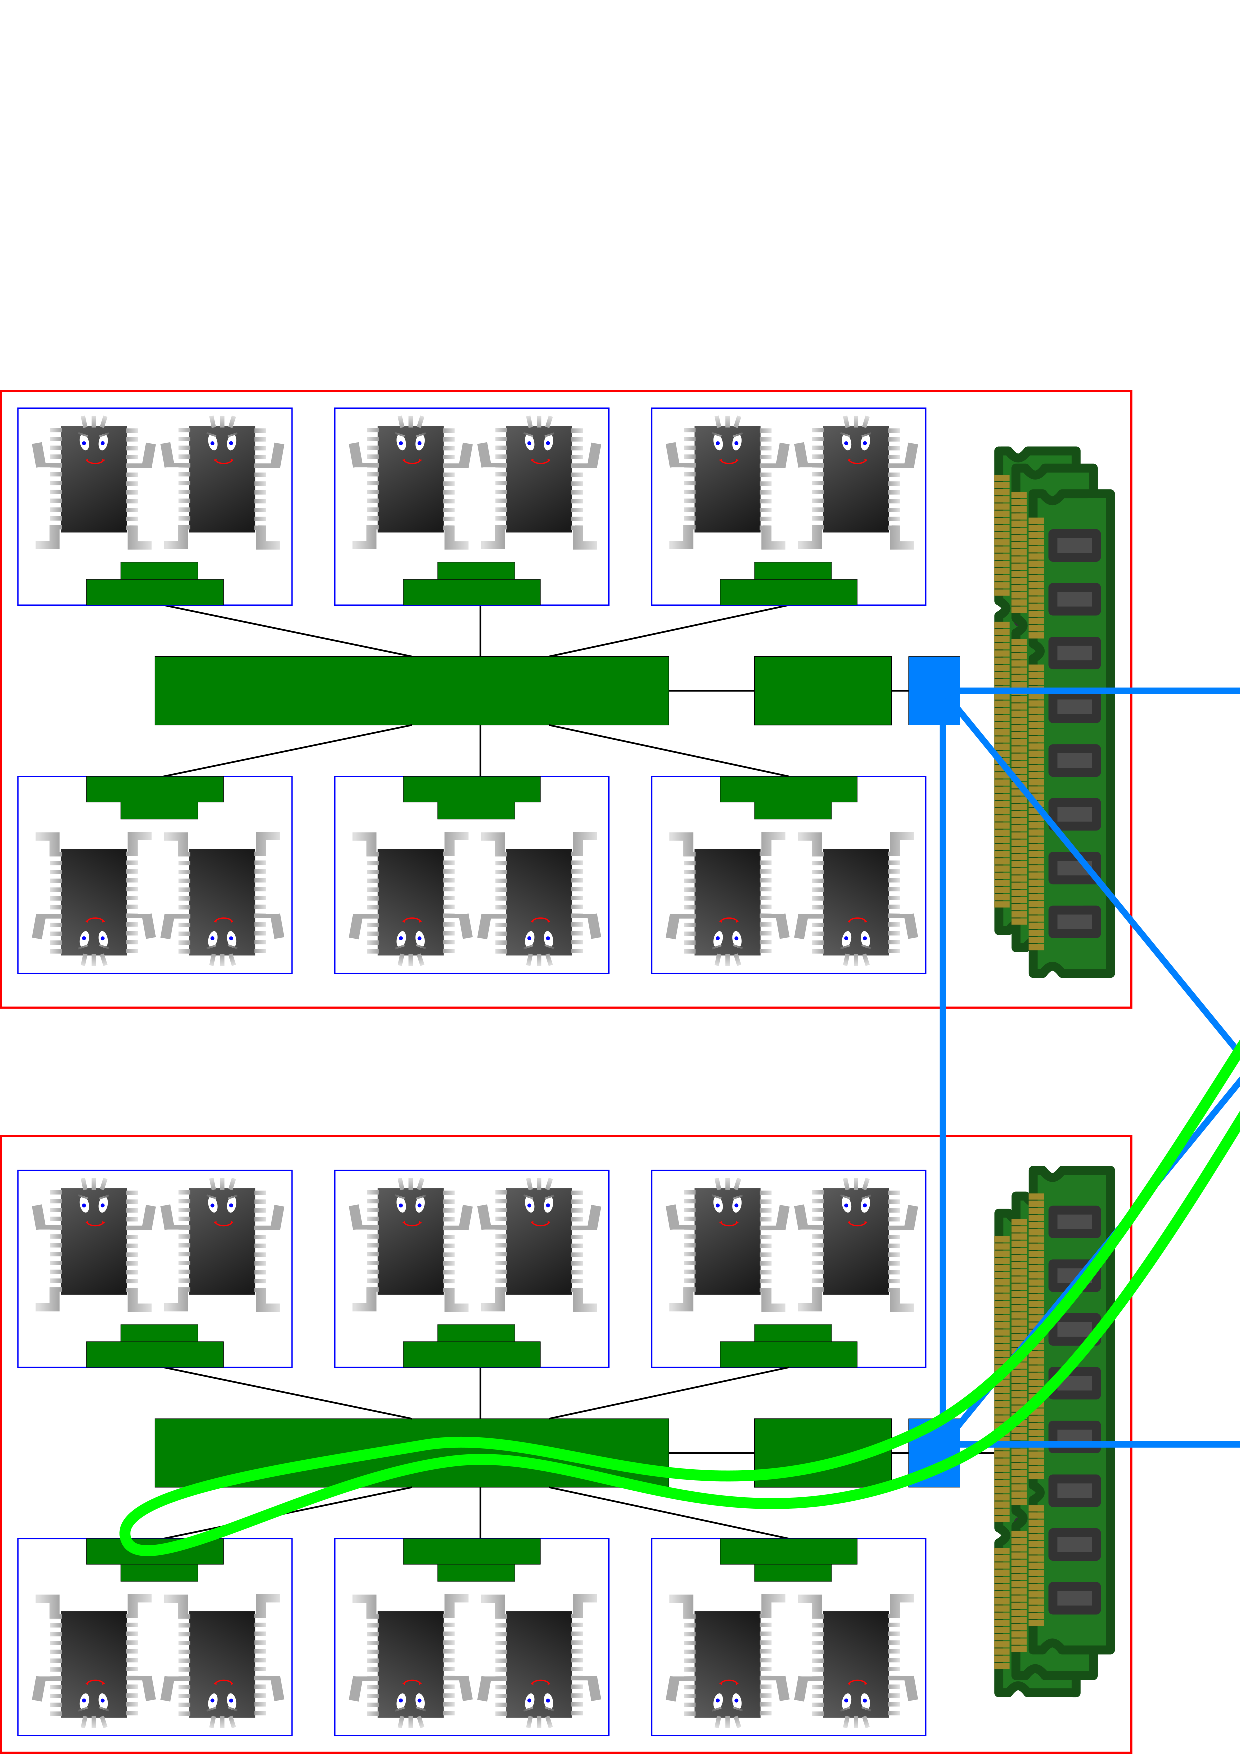
\includegraphics[width=0.4\textwidth]{out/pdf/svg/cache_coherent_read.pdf}}
\end{center}
\end{frame}

\newcommand{\Mbox}{{\textcolor{green}{\rule{3mm}{4mm}}}}
\newcommand{\Shbox}{{\textcolor{yellow}{\rule{3mm}{2.5mm}}}}
\newcommand{\Ibox}{{\textcolor{red}{\rule{3mm}{1mm}}}}

%%%%%%%%%%%%%%%%%%%%%%%%%%%%%%%%%% 
\begin{frame}
\frametitle{An example protocol : the MSI protocol}
\begin{itemize}
\item<1-> each line of a cache is inone of the following states

  \begin{center}
  {\em Modified} (\Mbox), {\em Shared} (\Shbox), {\em Invalid} (\Ibox)
  \end{center}
  
  \begin{itemize}
  \item<2-> Modified (\Mbox) $\iff$ you can \ao{read and write} the line without invoking a transaction
  \item<2-> Shared (\Shbox) $\iff$ you can \ao{read but not write} the line without invoking a transaction
  \item<2-> Invalid (\Ibox) $\iff$ you can \ao{neither read nor write} the line without invoking a transaction
  \end{itemize}
\end{itemize}
\end{frame}


%%%%%%%%%%%%%%%%%%%%%%%%%%%%%%%%%% 
\begin{frame}
\frametitle{An example protocol : the MSI protocol}
\begin{itemize}

\item<2-> a single address may be cached in multiple 
  caches (lines)

\item<3-> $\Rightarrow$ there are only two legitimate states for each line
  \begin{enumerate}
  \item<3-> one Modified \ao{\em (owner)} 
    $+$ others Invalid (\Ibox , \Mbox , \Ibox , \Ibox , \Ibox , \ldots)
  \item<4-> no Modified (\Shbox , \Ibox , \Shbox , \Shbox , \Ibox , \ldots)
  \end{enumerate}
\end{itemize}

\begin{center}
\only<1>{\includegraphics[width=0.6\textwidth]{out/pdf/svg/msi_0.pdf}}%
\only<2>{\includegraphics[width=0.6\textwidth]{out/pdf/svg/msi_1.pdf}}%
\only<3>{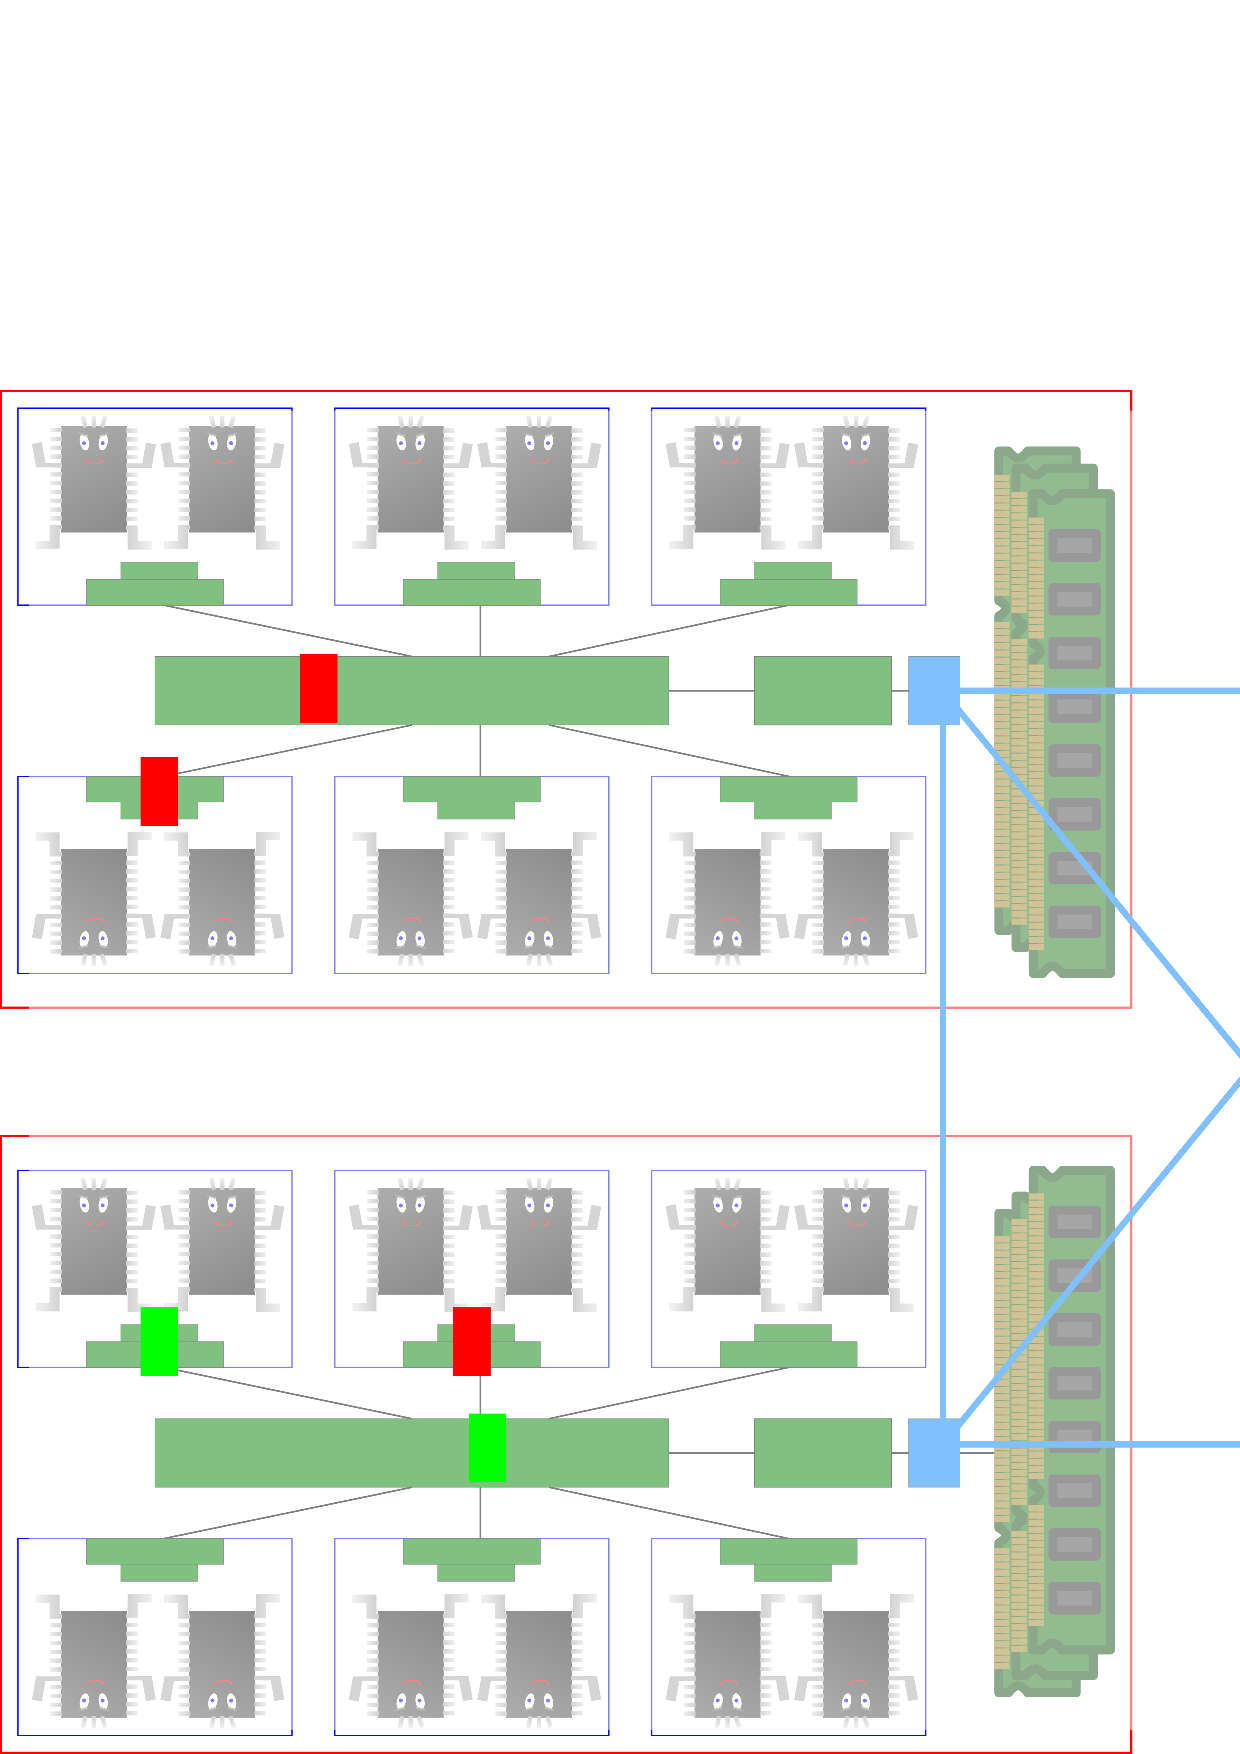
\includegraphics[width=0.6\textwidth]{out/pdf/svg/msi_2.pdf}}%
\only<4>{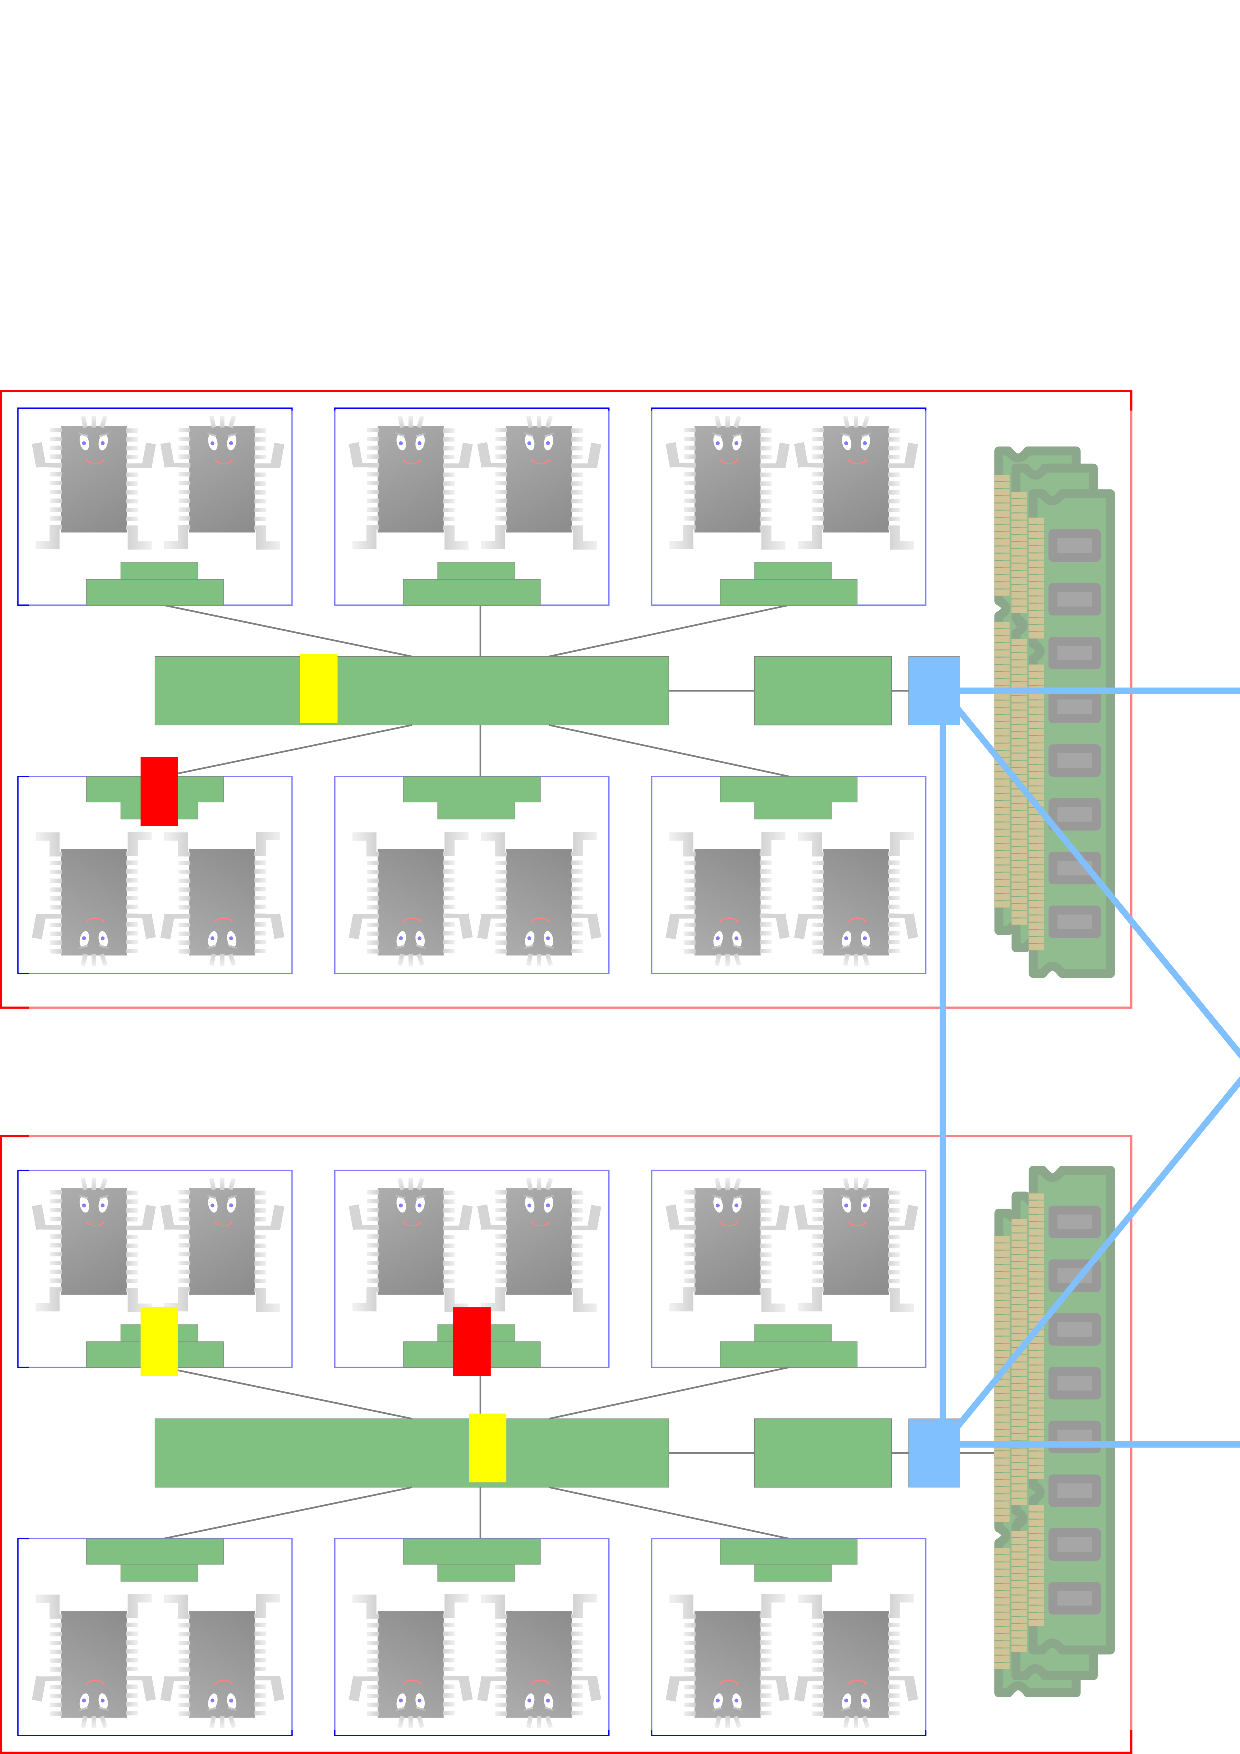
\includegraphics[width=0.6\textwidth]{out/pdf/svg/msi_3.pdf}}%
\end{center}

\end{frame}

%%%%%%%%%%%%%%%%%%%%%%%%%%%%%%%%%% 
\begin{frame}
\frametitle{Cache states and transaction}

\begin{itemize}
\item suppose a processor reads or writes an address and
  finds a line caching it
\item what happens when the line is in each state:
\begin{tabular}{|c|c|c|c|}\hline
      & Modified & Shared     & Invalid   \\\hline
read  & hit      & hit        & \ao{read miss} \\
write & hit      & \ao{write miss} & \ao{read miss; write miss} \\\hline
\end{tabular}

\item<2-> \ao{read miss:} $\rightarrow$ 
  \begin{itemize}
  \item there may be a cache holding it in Modified state \ao{\em (owner)}
  \item searches for the owner and if found, downgrade it to Shared
  \item 
\Ibox , \Mbox , \Ibox , [\Ibox], \Ibox , \ldots
$\Rightarrow$ 
\Ibox , \Shbox , \Ibox , [\Shbox], \Ibox , \ldots
  \end{itemize}
\item<3-> \ao{write miss:} $\rightarrow$
  \begin{itemize}
  \item there may be caches holding it in Shared state \ao{\em (sharer)}
  \item searches for sharers and downgrade them to Invalid
  \item 
\Shbox , \Ibox , \Shbox , [\Shbox], \Ibox , \ldots
$\Rightarrow$ 
\Ibox , \Ibox , \Ibox , [\Mbox], \Ibox , \ldots
  \end{itemize}
\end{itemize}
\end{frame}

%%%%%%%%%%%%%%%%%%%%%%%%%%%%%%%%%% 
\begin{frame}
\frametitle{MESI and MESIF}
\begin{itemize}
\item<1-> exntensions to MSI have been commonly used
\item<2-> \ao{MESI:} MSI $+$ \ao{Exclusive (owned but not modified)}
  \begin{itemize}
  \item when a read request finds no other caches that have the line, it owns it as Exclusive
  \item Exclusive lines do not have to be written back to main memory when discarded
  \end{itemize}

\item<3-> \ao{MESIF:} MESI $+$ \ao{Forwarding (a cache responsible for forwarding a line)}
  \begin{itemize}
  \item used in Intel QuickPath
  \item when a line is shared by many readers, one is designated as the Forwarder
  \item when another cache requests the line, only the forwarder sends it 
    and the new requester becomes the forwarder
  \item (in MSI or MESI, all sharers forward it)
  \end{itemize}
\end{itemize}
\end{frame}



%%%%%%%%%%%%%%%%%%%%%%%%%%%%%%%%%% 
\begin{frame}[fragile]
\frametitle{How to measure communication latency?}
\begin{itemize}
\item measure ``ping-pong'' latency between two threads
\begin{lstlisting}
volatile long x = 0;
volatile long y = 0;
\end{lstlisting}
\begin{columns}
\begin{column}{0.4\textwidth}
\begin{lstlisting}
(ping thread)
for (i = 0; i < n; i++) {
  x = i + 1;
  while (y <= i) ; 
}    
\end{lstlisting}
\end{column}
\begin{column}{0.4\textwidth}
\begin{lstlisting}
(pong thread)
for (i = 0; i < n; i++) {
  while (x <= i) ; 
  y = i + 1;
}    
\end{lstlisting}
\end{column}
\end{columns}
\end{itemize}

\begin{center}
\def\svgwidth{0.8\textwidth}
\input{out/tex/svg/measure_comm.pdf_tex}  
\end{center}
\end{frame}

%%%%%%%%%%%%%%%%%%%%%%%%%%%%%%%%%% 
\begin{frame}
\frametitle{Environment}
\begin{itemize}
\item Skylake X Gold 6130 (``big'' partition of the IST cluster)
\item 2 hardware threads $\times$ 16 cores $\times$ 4 sockets 
  ($=$ 128 processors seen by OS)

\item ensure variables {\tt x} and {\tt y} 
  are at least 64 bytes apart
  (not on the same cache line)
\item bind both threads on specific processors
  by OpenMP environment variable {\tt OMP\_BIND\_PROC=true} 
\item try all combinations of threads
  (i.e., with $p$ threads, measure all the $p(p-1)$ pairs)
  and show a matrix
\end{itemize}
\end{frame}


\iffalse
%%%%%%%%%%%%%%%%%%%%%%%%%%%%%%%%%% 
\begin{frame}
\frametitle{Result}
\begin{itemize}
\item $(i,j)$ indicates the roundtrip latency (in clocks)
  between processor $i$ and $j$

  \begin{columns}
    \begin{column}{0.6\textwidth}
{\scriptsize\input{out/tex/gpl/haswell_comm_matrix.tex}}
    \end{column}
    \begin{column}{0.4\textwidth}
{\footnotesize
\begin{tabular}{|r|r|r|}\hline
src & dest & latency \\\hline
0 & 1-15   & $\approx$ 500 \\
0 & 16-31  & $\approx$ 1200 \\
0 & 32     & $\approx$ 50 \\
0 & 33-47  & $\approx$ 500 \\
0 & 48-63  & $\approx$ 1200 \\\hline
\end{tabular}}
    \end{column}
  \end{columns}

\item a beautiful pattern emerges which is obviously telling

\end{itemize}
\end{frame}

%%%%%%%%%%%%%%%%%%%%%%%%%%%%%%%%%% 
\begin{frame}
\frametitle{Result}
\begin{columns}
\begin{column}{0.5\textwidth}
  \begin{itemize}
  \item e.g., which processor is ``close'' to processor $0$?
    \begin{itemize}
    \item 32 is closest
    \item 1-15 and 33-47 are close
    \item 16-31 and 48-63 are farthest
    \end{itemize}

  \item a natural interpretation
    \begin{itemize}
    \item $x$ and $(x+32)$ are two hardware threads on a core
    \item 0-15 are 16 cores on a socket
    \end{itemize}
  \item latencies
{\footnotesize
\begin{tabular}{|r|r|r|}\hline
hwts within a core & 50 \\
cores within a socket & 500 \\
across sockets & 1200 \\\hline
\end{tabular}}
  \end{itemize}
\end{column}
\begin{column}{0.5\textwidth}
%{\scriptsize\input{out/tex/gpl/magellan_comm_matrix.tex}}
{\scriptsize\input{out/tex/gpl/haswell_comm_matrix.tex}}
\end{column}
\end{columns}
\end{frame}



\fi

%%%%%%%%%%%%%%%%%%%%%%%%%%%%%%%%%% 
\begin{frame}
\frametitle{Result}
\begin{itemize}
\item $(i,j)$ indicates the roundtrip latency (in reference clocks)
  between processor $i$ and $j$ 

  \begin{columns}
    \begin{column}{0.6\textwidth}
%{\scriptsize\input{out/tex/gpl/skylake_comm_matrix.tex}}
    \end{column}
    \begin{column}{0.4\textwidth}
{\footnotesize
\begin{tabular}{|r|r|r|}\hline
src & dest & latency \\\hline
0 & 1-15   & $\approx$ 800 \\
0 & 16-63  & $\approx$ 1100 \\
0 & 64     & $\approx$ 110 \\
0 & 65-79  & $\approx$ 450 \\
0 & 80-127  & $\approx$ 1100 \\\hline
\end{tabular}}
    \end{column}
  \end{columns}

\item a beautiful pattern emerges which is obviously telling

\end{itemize}
\end{frame}

%%%%%%%%%%%%%%%%%%%%%%%%%%%%%%%%%% 
\begin{frame}
\frametitle{Result}
\begin{columns}
\begin{column}{0.5\textwidth}
  \begin{itemize}
  \item e.g., which processor is ``close'' to processor $0$?
    \begin{itemize}
    \item 64 is closest
    \item 1-15 and 65-79 are close
    \item 16-63 and 80-127 are farthest
    \end{itemize}

  \item a natural interpretation
    \begin{itemize}
    \item $x$ and $(x+64)$ are two hardware threads on a core
    \item 0-15 (and 65-79) are the 16 physical cores (32 hwts)
      on a socket
    \item others are on different sockets
    \end{itemize}
    
%   \item latencies
% {\footnotesize
% \begin{tabular}{|r|r|r|}\hline
% hwts within a core & 110 \\
% cores within a socket & 500-800 \\
% across sockets & 1100 \\\hline
% \end{tabular}}
  \end{itemize}
\end{column}
\begin{column}{0.5\textwidth}
% {\scriptsize\input{out/tex/gpl/skylake_comm_matrix.tex}}
\end{column}
\end{columns}
\end{frame}

%%%%%%%%%%%%%%%%%%%%%%%%%%%%%%%%%% 
\begin{frame}[fragile]
  \frametitle{What they imply to parallel algorithms?}
  \begin{itemize}
  \item you do not want to have many threads concurrently
    updating the same data
  \item remember SpMV COO?
\begin{lstlisting}
// assume inside @\ao{\tt \#pragma omp parallel}@
   ...
@\aka{\tt \#pragma omp for}@
for (k = 0; k < A.nnz; k++) {
  i,j,Aij = A.elems[k];
#pragma omp atomic  
  @\aka{\tt y[i]}@ += Aij * x[j];
}
\end{lstlisting}

\item {\aka{\tt y[i] +=}} may be costing
  1000 cycles when its single-thread execution
  would take just dozens of cycles
  \end{itemize}
\end{frame}

%%%%%%%%%%%%%%%%%%%%%%%%%%%%%%%%%% 
\begin{frame}
\frametitle{Summary (1): latency and bandwidth}

\begin{itemize}
\item \ao{latency} of data access heavily depends on which level of caches 
  you actually access:
  \begin{quote}
 L1 (a few cycles) $\leq$ main memory ($>$ 200 cycles)
  \end{quote}

\item a single core bandwidth is limited by:
\[ \frac{\mbox{cache line size} \times \mbox{LFB size}}{\mbox{latency}} \]

\item for main memory, it's much lower than what you see in the spec

\item max bandwidth is attainable only with multiple cores
\end{itemize}
\end{frame}


%%%%%%%%%%%%%%%%%%%%%%%%%%%%%%%%%% 
\begin{frame}
\frametitle{Summary (2): bandwidth differs by access patterns}
\begin{itemize}
\item 
\[ \mbox{bandwidth} = \frac{\mbox{line size} \times 
  \mbox{number of accesses in flight}}{\mbox{latency}} \]

\item \ao{bandwidth} heavily depends on the number of in-flight accesses,
  which depend on \ao{\emph{access patterns}}
  \begin{itemize}
  \item random address pointer chasing
  \item random but independent addresses
  \item sequential
  \end{itemize}
\end{itemize}
\end{frame}


%%%%%%%%%%%%%%%%%%%%%%%%%%%%%%%%%% 
\begin{frame}
\frametitle{Common misunderstanding}

\begin{itemize}
\item pointer chasing is always bad
  \begin{itemize}
  \item not when data fit in L1 (perhaps L2) cache
  \item not when accessed addresses are sequential
  \item not when you manage to chase many pointer chains
  \end{itemize}

\item random access is always worse than sequential access
  \begin{itemize}
  \item not so much when an element $\approx$ cache size
  \end{itemize}
\end{itemize}

\end{frame}

%%%%%%%%%%%%%%%%%%%%%%%%%%%%%%%%%% 
\begin{frame}
\frametitle{Summary (3): inter processor communication}
\begin{itemize}
\item cores communicate as a side effect of memory accesses (cache misses)

\item it is natually as expensive as L2/L3 misses (or more), depending on 
  whom you communicate with

\item shared memory is nice, but you cannot forget the cost
\end{itemize}
\end{frame}

\end{document}

%%%%%%%%%%%%%%%%%%%%%%%%%%%%%%%%%% 
\begin{frame}
\frametitle{Four types of cache misses}
\begin{itemize}
\item Compulsory:
  \begin{itemize}
  \item any address accessed misses on the first access
  \item in other words, misses that occur even with infinite caches
  \end{itemize}
\item Capacity
  \begin{itemize}
  \item if you access distinct addresses more than cache capacity, some of them must miss
  \item misses that occur with fully associative caches
  \end{itemize}
\item Conflict
  \begin{itemize}
  \item in $K$-way set associative cache, 
  \end{itemize}

\item Coherence
  \begin{itemize}
  \item read
  \item write
  \end{itemize}
\end{itemize}
\end{frame}


\end{document}
